%compiling with XeLaTeX
\documentclass[abstracton,
			   twoside,
			   openright,
			   parskip=half,
			   11pt]{scrreprt}
			   
%Presettings			   
%Personel Data
\title{Functional Renormalization and Quantum Gravity}
\author{Mathieu Kaltschmidt}
\date{\today}

%Statements
\newtheorem{statements}{Statements}[chapter]

%Page Layout and geometry
\usepackage{fancyhdr}
\fancyhfoffset{0pt}

\usepackage[a4paper,
			width = 150mm,
			top = 30mm,
		    bottom=30mm%,
		    %bindingoffset = 7mm
		    ]{geometry}
\usepackage[onehalfspacing]{setspace}


%Empty ages At The Beginning Of The Document
\def\blankpage{%
	\clearpage%
	\thispagestyle{empty}
	\addtocounter{page}{-1}
	\null%
	\clearpage}

%Renewing marks for appearance in header
\renewcommand{\chaptermark}[1]{
    \markboth{\mbox{\@chapapp}\ \thechapter.\ \ #1}{}%
}
\renewcommand{\sectionmark}[1]{
    \markright{\thesection\ \ #1}{}
}

%Chapter Layout
\KOMAoption{chapterprefix}{true}
\renewcommand*\raggedchapter{\centering}
\RedeclareSectionCommand[beforeskip=0pt,afterskip=\baselineskip]{chapter}
\setkomafont{chapterprefix}{\Large\mdseries}
\renewcommand*{\chapterformat}{%
  \chapappifchapterprefix{\nobreakspace}\thechapter\autodot%
  \IfUsePrefixLine{%
    \par\nobreak\vspace{-\parskip}\vspace{-.6\baselineskip}%
    \rule{0.9\textwidth}{0.5pt}\vspace{-1\baselineskip}%
  }{\enskip}%
}
\renewcommand\chapterlineswithprefixformat[3]{%
#2#3
}


%Page Layout For Beginning Of Chapter
\fancypagestyle{plain}{%
	\fancyhf{}  %clear all header and footer fields
	\fancyfoot[C]{- \thepage\hspace{3pt}-}
	\renewcommand{\headrulewidth}{0pt}
	\renewcommand{\footrulewidth}{0pt}
	}

%Page Layout For Other Pages
\pagestyle{fancy}
	\fancyhf{}
	\fancyhead[LE]{\footnotesize\nouppercase{\leftmark}}
	\fancyhead[RO]{\footnotesize\nouppercase{\rightmark}}
	\fancyfoot[C]{-\thepage-}
	\renewcommand{\headrulewidth}{0.2pt}
	\renewcommand{\footrulewidth}{0pt}

%Headings
\setkomafont{section}{\textsf\bfseries\Large}
\setkomafont{subsection}{\textsf\bfseries\large}
\setkomafont{subsubsection}{\textsf\bfseries\normalsize}


%Math and Units
\usepackage{amsmath, amssymb, commath, mathtools}
\usepackage{physics}
\usepackage[hyperref]{ntheorem}
\usepackage{xfrac}
\usepackage[separate-uncertainty]{siunitx}


%Tables
\usepackage{array} %math mode in tables
\usepackage{booktabs} %hline rules

%Language Settings and Microtype
\usepackage{fontspec, xunicode}
\usepackage[utf8]{inputenc}
\usepackage{lmodern}
\setmainfont{Palatino}
\setsansfont{Optima}
\setmonofont[Scale=MatchLowercase]{Menlo}
\usepackage{polyglossia}
\setmainlanguage{english}
\setotherlanguages{german, french}
\usepackage{microtype}

%Useful Packages
\usepackage{graphicx} %including images
\usepackage{float} %better positioning for float environments
\usepackage{blindtext} %for testing the output
\usepackage[labelfont=bf]{caption} %nice captions
\usepackage{subcaption} %for multiple plots

%TikZ and Feynman Diagrams
\usepackage{tikz}
\usepackage{tikz-feynman}
\tikzfeynmanset{compat=1.0.0}
\usetikzlibrary{external}
	\immediate\write18{mkdir -p feynman-diagrams}
	\tikzexternalize[
  	prefix=feynman-diagrams/,
  	system call={
    lualatex \tikzexternalcheckshellescape -halt-on-error -interaction=batchmode -jobname="\image" "\texsource"  || rm "\image.pdf"},
	]

%Appendix and Bibliography
\RequirePackage[toc,page]{appendix}

\usepackage[
	style=numeric-comp,
	backend=biber,
	isbn=false,
	date=year,
	url=false,
	doi=false
]{biblatex}
\addbibresource{bib/bsc.bib}

%Colorlinks etc.
\usepackage[colorlinks=False]{hyperref}
\hypersetup{allcolors=BScBlue}

%Statement environment
\newcommand{\statement}[1]{\stepcounter{statements}\begin{center}
	\textbf{#1}
	\end{center}
}

%Color Settings
\usepackage{xcolor}
\definecolor{BScRed}{RGB}{157,0,0}
\definecolor{BScBlue}{RGB}{1,1,141}
\definecolor{BScGreen}{RGB}{0, 119, 85}
\definecolor{BScGray}{RGB}{102, 102, 142}

%Useful definitions

\newcommand{\Z}{\mathcal{Z}[J]}
\renewcommand{\S}{\mathcal{S}[\varphi]}
\newcommand{\D}{\mathcal{D}}
\newcommand{\W}{\mathcal{W}[J]}
\newcommand{\cf}[1]{\langle #1 \rangle}


\newcommand{\Ricci}{\mathcal{R}}
\newcommand{\Gammak}{\Gamma_{k}}
%\newcommand{\Gamma2}{\Gamma^{(2)}_{k}}
\newcommand{\Lambdak}{\Lambda_k}
\renewcommand{\tr}[1]{\operatorname{Tr}\left[ #1 \right]}
%\renewcommand{\baselinestretch}{1.5}
\begin{document}

\pagenumbering{roman}
%Introductory stuff, abstracts and toc

{\hypersetup{allcolors=black}
\begin{titlepage}

	\begin{center}
		\makeatletter
		\vspace{2cm}
		\Large\textbf{Department of Physics and Astronomy\\
			Heidelberg University}
		
		%\vspace{13cm}
		\vfill
		\normalsize
		Bachelor thesis in Physics\\
		\normalsize
		submitted by\\[0.4cm]
		\Large
		\textbf{\@author}\\[0.4cm]
		\normalsize
		from Kappel-Grafenhausen \\ [0.4cm]
		\Large\textbf{2019}

		\cleardoublepage
		\thispagestyle{empty}
		\LARGE\textbf{\@title}\\[.4cm]

		\vfill
		\normalsize
		This Bachelor thesis has been carried out by \\ 
		\vspace{3pt}
		\textbf{\@author}  \\ 
		\vspace{3pt}
		at the\\
		\vspace{3pt}
		\textbf{Institute for Theoretical Physics} \\ at \\\textbf{Heidelberg University}\\
		\vspace{5pt}
		under the supervision of\\
		\vspace{5pt}
		\textbf{Prof. Dr. Jan M. Pawlowski}
		
		\makeatother
	\end{center}
\cleardoublepage
\end{titlepage}}
{\hypersetup{allcolors=black}
\thispagestyle{plain}

\makeatletter

\begin{center}
\textbf{\large\@title} \\
\vspace{.1cm}
\@author \\
\end{center}

\makeatother

%Abstract in english language
\statement{\large Abstract}
In this work we discuss the Asymptotic Safety approach as a possible realization of a theory of quantum gravity based on path integral quantization using functional renormalization group methods. First, the exact renormalization group equation is solved in a spin-2 graviton approximation using the background field formalism and the respective fixed point structure is analyzed. In the second part, we investigate minimally coupled scalar, fermion and gauge fields and their impact on the system. Finally, we discuss the validity of our computations in the background field method and present the fluctuation field formalism as a modern, alternative approach. 

\vfill

%Abstract in german language
\begin{otherlanguage}{german}
\statement{\large Zusammenfassung}
In dieser Arbeit wird der Asymptotic-Safety Zugang als m\"oglicher Ansatz zur Realisierung einer Theorie der Quantengravitation im Rahmen der Pfadintegral-Quantisierung mit Methoden der funktionalen Renormierungsgruppe untersucht. Die exakte Renormierungsgruppengleichung wird zun\"achst in einer Spin-2-Graviton N\"aherung im Hintergrundformalismus gel\"ost und die resultierende Fixpunkt-Struktur analysiert. Im zweiten Teil der Arbeit wird der Einfluss von minimal gekoppelten Skalar-, Fermion- und Eichfeldern auf das System \"uberpr\"uft. Abschlie\ss end wird die Hintergrundfeld-Methode kritisch hinterfragt und mit der Fluktuationsfeld-Methode ein moderner, alternativer Zugang pr\"asentiert.
\end{otherlanguage}
\vfill
\cleardoublepage}

{\hypersetup{linkcolor=black}
\tableofcontents  
}
\cleardoublepage


\setcounter{tocdepth}{1}
\pagenumbering{arabic}

%Main part
	\chapter{Introduction}
Einsteins theory of General Relativity successfully describes gravitational phenomena ranging from quotidian physics to the dynamics of whole galaxies very precisely in terms of the geometry of spacetime. This high precision has been proved once again recently in 2016, with the first observation of gravitational waves by the LIGO and VIRGO collaborations \cite{LIGO2016}. Nevertheless, General Relativity is a \textit{classical} field theory and it is assumed, that the theory breaks down at some characteristic energy scale, i.\,e. the Planck scale
\begin{equation*}
	\Lambda_{\text{Planck}} \approx 10^{19} \ \text{GeV}. 
\end{equation*}
For decades, physicists have been working on finding a microscopic,  \textit{quantum} theory of gravity, comparable to the successful description of the other three fundamental forces, namely the electromagnetic, the weak- and the strong nuclear forces, all unified in the Standard Model of Particle Physics. Such a quantum theory of gravity could provide interesting insides into the physics of e.\,g. the early universe or black holes. Among the most popular proposals for such a theory are e.\,g. String Theory or Loop Quantum Gravity. \\
 One of the main problems in verifying predictions from such theories is, that currently it is all but impossible to probe (quantum) gravitational effects at energies near $\Lambda_{\text{Planck}}$. Particle colliders such as the Large Hadron Collider (LHC) nowadays reach maximum center-of-mass energies of about $\sqrt{s} \approx 14 \ \text{TeV} = 14\cdot 10^3 \ \text{GeV}$. In addition to this experimental problem, it is well known, that the quantization of General Relativity leads to a (perturbatively) non-renormalizable theory  due to the negative mass dimension of Newtons constant
\begin{equation*}
	[G] = -2  
\end{equation*}
in $d=4$ spacetime dimensions \cite{GoroffSanotti1985, tHooftVeltmann1974}. During the last decades, the mathematical toolkit for theoretical physicists has evolved quite rapidly. Especially the development of the Functional Renormalization Group, in its modern formulation introduced by Kenneth Wilson in 1971 \cite{Wilson1971}, offers a powerful, non-perturbative tool to solve path integrals in quantum field theory. \\
Proposed by Steven Weinberg in 1978 \cite{Weinberg1980}, the Asymptotic Safety scenario for Quantum Gravity provides a mechanism for constructing a fundamental quantum field theory of gravity in the language of the Functional Renormalization Group. It aims at generalizing the concept of Asymptotic Freedom, well-known e.\,g. in the context of Yang-Mills theories. The basic idea is, that the ultraviolet (= high energy) behavior of gravity may be governed by a Non-Gaussian Fixed Point (NGFP) of the underlying renormalization group flow. A first successful study of quantum gravity within the Asymptotic Safety scenario was conducted by Martin Reuter in 1996 \cite{Reuter1996}. He derived the flow equations and proved the existence of such a NGFP in a pure-gravity setting in a truncated subsystem. The so-called Einstein-Hilbert truncation he employed back then, will also be the truncation of our choice for this work. \\
This thesis aims at investigating quantum gravity within the Asymptotic Safety scenario in the Einstein-Hilbert truncation after introducing the concepts needed for a general understanding of the subject. To get a first insight into the underlying structures, the theory is solved in a pure-gravity setting within a transverse-traceless spin-two graviton approximation. In order to probe a more realistic situation, the gravity-matter sector of the theory has to be taken into account. We include minimally coupled matter fields,  i.\,e. scalar, fermionic and gauge fields and study their impact on the underlying fixed point structure of the Einstein-Hilbert truncation. Earlier studies put rather strict constraints on the matter content compatible with Asymptotic Safety, see e.\,g. \cite{DonaEichhornPercacci2013}. In more recently published  research papers, e.\,g. in \cite{MeibohmPawlowskiReichert2015, ChristiansenLitimPawlowskiReichert2018}, strictly less severe constraints have been proposed. The latter results are based on calculations involving a vertex expansion of the effective average action. The flow of the couplings is then obtained from the flow of the $n$-point functions.
 Throughout this work, all computations will be performed in a background field approximation. Since this approximation has to be treated with care, we have to critically review our computations at the end of the thesis. \\
 
The structure of this work is the following: In chapter \ref{chap:QFT} the field theoretical language and the Functional Renormalization Group (FRG) are introduced. A derivation of Wetterich's exact renormalization group equation, a.\,k.\,a. the flow equation,  completes our discussion of non-perturbative approaches to quantum field theory. Chapter \ref{chap:GR} provides the background knowledge on gravity and curved spacetimes. In chapter \ref{chap:EHT}, as a first step towards quantum gravity, the Asymptotic Safety approach is motivated and the flow equation is solved within the Einstein-Hilbert truncation in a transverse-traceless spin-two graviton approximation. The inclusion of matter is studied in chapter \ref{chap:Matter}. In chapter \ref{chap:BGindependence} we critically review the background field approximation.
To conclude this work, the results are summarized and discussed in chapter \ref{chap:Conclusion}. \\
 Throughout this thesis we use natural units such that $\hbar = c  \equiv 1$. Einsteins sum convention is implicitly understood: Whenever an index appears twice in a single term, summation of that term over the whole index range is implied unless stated otherwise. As usual, greek indices refer to some $d$-dim. spacetime coordinates, ranging from $0$ to $d-1$, i.\,e. $x^{\mu} = (x^0, x^1, \cdots, x^{d-1})$. Unless stated otherwise, we work in $d=4$ spacetime dimensions.


	\chapter{Functional Methods in Quantum Field Theory}\label{chap:QFT}
This chapter introduces a treatment of quantum field theory using functional methods. The main goal is to become familiar with the physical concepts and the notation used throughout this work and to derive the flow equation for the average effective action, introduced by Christof Wetterich in 1993 \cite{Wetterich1992}. 
For the derivation of the flow equation we are following \cite{Gies2006, PawlowskiNPgaugeLecture}.

\section{Generating Functionals and Correlation Functions}
Consider a theory setting of $N$ real scalar fields $\varphi_a(x), a \in \{1,\dots,N\}$ in $d$-dimensional Euclidean space. The corresponding partition sum in presence of sources $J_a(x)$ reads
\begin{align}
	Z[J] = \frac{1}{\mathcal{N}} \int \D\varphi \operatorname{e}^{-\S + J\cdot\varphi}.
	\label{eqn:partition}
\end{align}
The action $\mathcal{S}$ is specified together with an ultraviolet cutoff scale $\Lambda$, later being the momentum scale where we initialize the flow equations and some normalization factor $\mathcal{N}$.\\
In this notation, the scalar product sums over field components and integrates over all space,
\begin{align}
	J\cdot\varphi = \int_x J_a(x) \ \varphi_a(x) = \int_p \tilde{J}_a(p) \ \tilde{\varphi}_a(p),
\end{align}
with
\begin{align}
\int_x = \int_{\mathbb{R}^d} \dd^d x \qquad \text{and} \qquad \int_p = \int_{\mathbb{R}^d} \frac{\dd^d p}{(2\pi)^d}.	
\end{align}

The partition sum $Z[J]$ is called a \textit{generating functional}. It directly allows us to compute field expectation values
\begin{align}
	\phi := \cf{\varphi} = \eval{\frac{1}{Z}\frac{\delta Z}{\delta J}}_{J=0} = \int \D\varphi \ \varphi \ \operatorname{e}^{-\S + J\cdot\varphi}
\end{align}
and higher order correlation functions
\begin{align}
\cf{\varphi(x_1) \cdots \varphi(x_n)} := \cf{\varphi^n} = \frac{1}{Z}\eval{\frac{\delta^n Z}{\delta^n J}}_{J=0} = \int \D\varphi \ \overbrace{\varphi_1 \cdots \varphi_n}^{:= \ \varphi^n} \ \operatorname{e}^{-\S + J\cdot\varphi}
\end{align}
via functional differentiation. This means, we are basically able to compute all contributing Feynman diagrams for our theory setting, if we have knowledge of its corresponding (grand) canonical partition sum. \\
 For a more efficient description of the theory in terms of only the \textit{connected} correlation functions, we define the \textit{Schwinger functional} $W[J]$ as the logarithm of $Z[J]$,  
\begin{align}
W[J] = \ln Z[J].
\label{eqn:Schwinger}
\end{align}
It is the generating functional for the connected correlation functions. The normalization factor $\mathcal{N}$, introduced in (\ref{eqn:partition}) enters here as an additive constant, which drops out for all higher order correlation functions, except for the zero-point function. This term is connected to the thermodynamic quantities of the system and becomes important, when external parameters such as temperature, volume or the chemical potential are varied. For the case of quantum gravity, it is linked to the cosmological constant $\Lambda$. Nevertheless, in general we are only interested in correlation functions with $n\geq 1$ and therefore we drop this term.\\
Consider for example the connected two-point function $G_{ab}(x,y) = G_{\alpha\beta}$\footnote{To save on notation, we introduce collective indices $\alpha = (x,a)$ or $(q,a)$ in momentum space.}, known as the propagator, correlating the field $\varphi_a$ at spacetime point $x$ with the field $\varphi_b$ at $y$,
\begin{equation}
\begin{aligned}
	G_{\alpha\beta} &= \frac{\delta^2W[J]}{\delta J_{\alpha}\delta J_{\beta}} = \frac{\delta}{\delta J_{\alpha}}\left(\frac{1}{Z}\frac{\delta Z}{\delta J_{\beta}}\right)  \\[10pt]
				&= \frac{1}{Z}\left(\frac{\delta^2Z}{\delta J_{\alpha}\delta J_{\beta}}\right) - \frac{1}{Z^2}\left(\frac{\delta Z}{\delta J_{\alpha}}\right)\left(\frac{\delta Z}{\delta J_{\beta}}\right)\\[10pt]
				&= \cf{\varphi_{\alpha}\varphi_{\beta}} - \phi_{\alpha}\phi_{\beta} = \cf{\varphi_{\alpha}\varphi_{\beta}}_{\text{c}}. 
\end{aligned}
\label{eqn:G_connected}						
\end{equation}
The propagator is the key object in functional approaches to quantum field theory. It depends on the chosen background via $J$. \\
It is still possible to make our computations even more efficient, because $W[J]$ still contains some redundant information. Connected correlation functions can be separated into so-called one-particle irreducible (1PI) and one-particle reducible ones. The 1PI correlation functions are those, whose corresponding Feynman diagrams can \textit{not} be separated into two disconnected ones by cutting a single internal line. As an example, contributing 1PI and reducible diagrams to the connected four-point function for Yukawa theory are depicted in figure (\ref{fig:1PI_Yukawa}). \\
\begin{figure}[t]
\centering
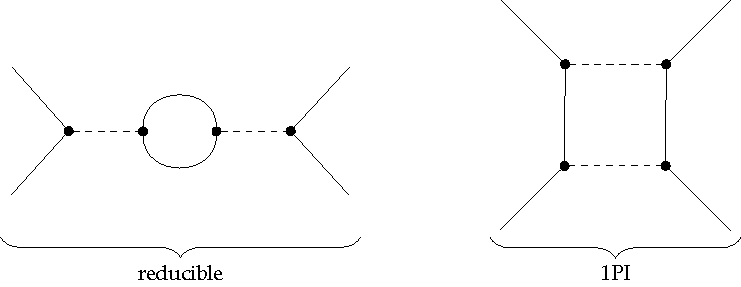
\includegraphics[width=0.8\textwidth]{figs/TikZ/1PI_Yukawa}
\caption[Contributing one-particle reducible and 1PI diagrams to the four-point-function in Yukawa theory]{Contributing one-particle reducible and 1PI diagrams to the four-point-function in Yukawa theory, inspired by \cite{FloerchingerWetterichQFT}.}	
\label{fig:1PI_Yukawa}
\hrulefill
\end{figure}
The generating functional for the  1PI correlation functions, the \textit{effective action} $\Gamma$, is obtained from the Schwinger functional via a Legendre transformation, 
\begin{equation}
	\Gamma[\phi]=\sup _{J}\left\{\int_{x} J(x) \phi(x)-W[J]\right\}=\int_{x} J_{\mathrm{sup}}(x) \phi(x)-W\left[J_{\mathrm{sup}}\right],
\label{eqn:Def_Gamma}
\end{equation}
where $J_{\mathrm{sup}}$ has to be understood as a field-dependent current $J_{\mathrm{sup}}[\phi]$. In the following, we will drop the subscript, its meaning is implicitly understood. 
The quantum equation of motion derived from $\Gamma$ reads
\begin{align}
	J(x) = \frac{\delta\Gamma[\phi]}{\delta\phi(x)}.
	\label{eqn:quantum_eom}
\end{align}
It allows us to understand the dynamics of field expectation values, taking the effects of all quantum fluctuations into account.
From a physical point of view, the effective action $\Gamma$ is the quantum analogue of the classical action $\mathcal{S}$. The performed Legendre transformation leads us to a mean field description of our theory with $\phi = \cf{\varphi}$ on a given background, as introduced before. The symmetries of the classical action are in general still present in the effective action.\\
In terms of the effective action, higher order correlation functions are again obtained by performing functional derivatives, but now w.\,r.\,t. the mean field $\phi$,
\begin{align}
	\Gamma^{(n)}\left(x_{1}, \ldots, x_{n}\right)=\frac{\delta^{n} \Gamma}{\delta \phi\left(x_{1}\right) \cdots \delta \phi\left(x_{n}\right)}.
\end{align}
With the definition of the effective action (\ref{eqn:Def_Gamma}), we find
\begin{equation}
	\operatorname{e}^{-\Gamma[\phi]}=\int_{\Lambda} \mathcal{D} \varphi \exp \left(-\mathcal{S}[\phi+\varphi]+\int_x \frac{\delta \Gamma[\phi]}{\delta \phi(x)} \varphi(x)\right).
\end{equation}  
The solution of such functional integro-differential equations is highly non-trivial. To solve this problem, we want to make use of the Functional Renormalization Group. The general idea of this approach is to introduce a scale-dependent action $\Gamma_k$, interpolating between the bare, microscopic action $\mathcal{S}$ and the full quantum effective action $\Gamma$. A more formal motivation and a derivation of the equation governing this interpolation process is presented in the next section.   
 \section{Functional Renormalization Group}
The Functional Renormalization Group (FRG) is a mathematical tool, allowing us to investigate the dynamics of physical systems on different energy (momentum) scales. This idea is based on a continuous version of Leo P. Kadanoff's block spin model on the lattice \cite{Kadanoff1966} and was developed by Kenneth G. Wilson in 1971 \cite{Wilson1971}. It aims at solving the theory by integrating successively momentum shell by momentum shell, being the reason why the path integral approach to quantum field theory provides a suitable framework. The main advantage of the FRG approach is, that no regularization or renormalization procedure has to be applied. The latter one is already implemented systematically, which secures the self-consistency of the approach. As this section is only supposed to introduce the basics of the FRG, we refer the interested reader to more complete reviews, e.\,g. \cite{Pawlowski2005, Gies2006}, particularly for applications in different areas of physics.

As a first step towards a FRG equation we need to introduce an infrared cutoff scale $k$ in our theory, below which the modes are not integrated out. A common way to introduce such a scale is by  adding a scale-dependent cutoff term $\Delta\mathcal{S}_k$ in the definition of the partition sum (\ref{eqn:partition}) and therefore automatically also in the definition of the Schwinger functional (\ref{eqn:Schwinger}):
\begin{align}
W_{k}[J]=\ln Z_{k}[J]=\ln \int \mathcal{D} \varphi  \operatorname{e}^{-\mathcal{S}[\varphi]+J \cdot \varphi-\Delta \mathcal{S}_{k}[\varphi]}.
\label{eqn:Wk}
\end{align}
The physical scale $k$ we introduced here is known as \textit{renormalization scale} and has units of inverse length, meaning large $k$ correspond to small distances and vice versa. The cutoff term $\Delta\mathcal{S}_k$ is a quadratic functional depending on the field $\varphi$:
\begin{align}
	\Delta \mathcal{S}_{k}[\varphi]=\frac{1}{2} \varphi \cdot R_{k} \cdot \varphi=\frac{1}{2} \int_{x, y} \varphi_{\alpha} \ R_{k, \alpha\beta} \ \varphi_{\beta}.
\end{align}
The function $R_k$ is called \textit{regulator}. It plays an important role for this formulation of quantum field theory. The regulator is chosen such that only the propagation for momentum modes with $p^2 \lesssim k^2$ is suppressed. The most important physical limits are summarized in the following:
\begin{align}
	R_{k}(p^2) \rightarrow\left\{\begin{array}{ll}{k^{2}} & {\text { for } p \rightarrow 0} \\ {0} & {\text { for } p \rightarrow \infty} \\ {0} & {\text { for } k \rightarrow 0} \\ {\infty} & {\text { for } k \rightarrow \Lambda}\end{array}\right.
\label{eqn:regulator_limits}
\end{align}
A convenient choice of the regulator is given by
\begin{align}
	R_k(p^2) = p^2 \cdot r_k(y),
\end{align}
with $ y := \frac{p^2}{k^2}$, and a dimensionless regulator shape function $r_k$, only depending on the dimensionless momentum ratio $y$. There is a plethora of different types of shape functions, but for the computations performed in this work we restrict ourselves to a class of rather simple, so-called Litim-type regulators with shape functions
\begin{align}
r_k(y) = \left(\frac{1}{y} - 1\right)\theta(1-y),
\label{eqn:Litim}	
\end{align}
where $\theta$ is the Heaviside step function. This class of \textit{sharp} regulators is a good choice for finding analytic FRG equations in simple approximations. For numerical approaches, exponential regulators such as depicted in figure (\ref{fig:exp_regulator}) are well suited.\\
\begin{figure}[t]
\centering
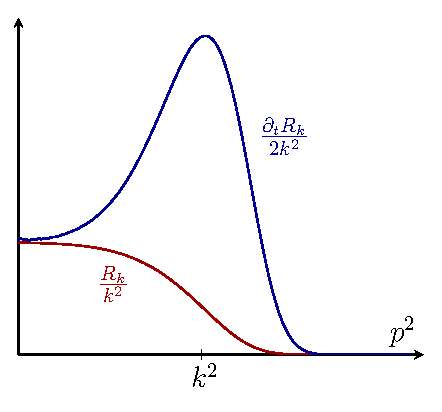
\includegraphics[width=0.4\textwidth]{figs/Plots/regulator_plot}
\caption[Shape of a typical exponential regulator function $R(p^2)$ and its derivative w.\,r.\,t. the RG time $t$.]{Shape of a typical exponential regulator function $R(p^2)$ and its derivative w.\,r.\,t. the RG time $t$. The regulator has a finite value for momenta smaller than $k^2$ and therefore acts as a suppressing mass term. The peak of $\partial_tR_k$ around $k^2=p^2$ clearly shows the implementation of Wilsons idea of shell-wise momentum integration.}	
\label{fig:exp_regulator}
\hrulefill
\end{figure}
At this point it is quite convenient to introduce the \textit{RG time} $t$ as
\begin{align}
	t = \ln\left(\frac{k}{\Lambda}\right) \qquad \longrightarrow\qquad \partial_t = \frac{\partial}{\partial\ln(k/\Lambda)} = \frac{k}{\Lambda}\frac{\partial}{\partial(k/\Lambda)} = k \partial_k,
\end{align}
where $\Lambda$ is a fixed reference scale. Usually one chooses the ultraviolet cutoff scale, where the flow is initialized.\\
In this setting, (\ref{eqn:Wk}) provides a good starting point for solving the theory by successively lowering the cutoff scale $k$ infinitesimally and integrating out all momentum modes $\varphi_{p\approx k}$. This procedure can be formalized by taking a scale derivative of our scale-dependent functional (\ref{eqn:Wk}):
\begin{equation}
\begin{aligned} \partial_{t} W_{k}[J] &=-\frac{1}{2} \int \mathcal{D} \varphi \ \varphi(-p) \partial_{t} R_{k}(p) \varphi(p) \operatorname{e}^{-\mathcal{S}[\varphi]+ J \cdot\varphi - \Delta \mathcal{S}_{k}[\varphi]} \\ &=-\frac{1}{2} \int_p \partial_{t} R_{k}(p) G_{k}(p)+\partial_{t} \Delta S_{k}[\phi], 
\label{eqn:dtW}
\end{aligned}
\end{equation}
where we used the definition of the connected propagator:
\begin{equation}
G_k = \frac{\delta^2 W_k[\phi]}{\delta\phi(x)\delta\phi(y)}.
\label{eqn:Gk}
\end{equation}
The \textit{flowing} or \textit{effective average action} $\Gamma_k$ is then again defined via a modified Legendre transformation, including the insertion of $\Delta S_k$:
\begin{equation}
	\Gamma_{k}[\phi]=\sup _{J}\left(\int_x J(x) \phi(x)-W_{k}[J]\right)-\Delta S_{k}[\phi].
\end{equation}
This yields the modified, scale-dependent quantum equation of motion:
\begin{align}
	J(x) = \frac{\delta\Gamma_k[\phi]}{\delta\phi(x)} + \left(R_k\phi\right)(x).
\end{align}
Compared to the scale-independent version (\ref{eqn:quantum_eom}), we find an additional, regulator dependent term, but with the properties of the regulator presented in (\ref{eqn:regulator_limits}) in mind, we see that in the limit $k\rightarrow 0 $ the initial equation of motion is restored.
We find
\begin{equation}
	\frac{\delta J(x)}{\delta \phi(y)}=\frac{\delta^{2} \Gamma_{k}[\phi]}{\delta \phi(x) \delta \phi(y)}+R_{k}(x, y).\label{eqn:dJdphi}
\end{equation}
With the help of these relations we are able to show that 
\begin{equation}
\begin{aligned} \delta\left(x-x^{\prime}\right) =\frac{\delta J(x)}{\delta J\left(x^{\prime}\right)}&=\int_y \frac{\delta J(x)}{\delta \phi(y)} \frac{\delta \phi(y)}{\delta J\left(x^{\prime}\right)} \\[10pt] &=\int_y\left(\Gamma_{k}^{(2)}[\phi]+R_{k}\right)(x, y) \ G_{k}\left(y-x^{\prime}\right).
\end{aligned}
\end{equation}
Here, we used (\ref{eqn:dJdphi}) and the definition of $G_k$ (\ref{eqn:Gk}). 
This yields the following important identity:
\begin{equation}
	G_k = \left(\Gamma_k^{(2)} + R_k\right)^{-1}.
	\label{eqn:inverse_prop_identity}
\end{equation}
Altogether, we arrive at the \textit{flow equation}, a.\,k.\,a. the \textit{Wetterich equation} for the average effective action:
\begin{equation}
\begin{aligned}
\partial_t \Gamma_k[\phi] &\overset{\phantom{(\ref{eqn:dtW})}}{=} -\partial_t W_k +\int\left(\partial_t J\right) \phi - \partial_t \Delta S_k[\phi] = - \partial_t W_k[J] - \partial_t \Delta S_k[\phi] \\[5pt] 
&\overset{(\ref{eqn:dtW})}{=} \frac{1}{2} \int_p G_{k}(p) \ \partial_{t} R_{k}(p)\\[5pt]
&\overset{(\ref{eqn:inverse_prop_identity})}{=}\frac{1}{2} \operatorname{STr}\left[\left(\Gamma_{k}^{(2)}[\phi]+R_{k}\right)^{-1}\partial_{t} R_{k}\right].
\end{aligned}
\label{eqn:Wetterich}
\end{equation}
The supertrace $\operatorname{STr}$ sums over all internal indices and integrates over momentum space. For Grassmann fields, it also involves the inclusion of a minus sign. We will drop the $\operatorname{S}$ for the rest of this work, its meaning should be understood implicitly.
The flow equation can be represented diagrammatically as a $1$-loop equation:
\begin{figure}[H]
\centering
\begin{gather}
\begin{aligned}
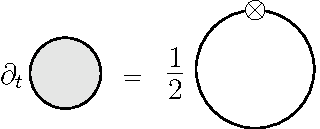
\includegraphics[scale=1.1]{figs/TikZ/wetterich_equation}
\end{aligned}
\end{gather}
\end{figure}
\vspace{-0.7cm}
The full propagator $\left[\Gamma_k^{(2)} + R_k\right]^{-1}$ is represented as usual as a single, double, dashed etc. line, dependent on the field content.
The crossed circle $\otimes$ denotes the insertion of the respective regulator or more precisely its derivative w.\,r.\,t. the RG time $t$. Here $\partial_{t} R_{k, ij}(p, q)=\partial_{t} R_{k}(p^2)(2 \pi)^{d} \  \delta_{i j} \ \delta(p-q)$ and therefore the trace on the r.\,h.\,s. effectively sums over just one index $i$ and integrates over one loop momentum $p$. \\
\begin{figure}[t]
\centering
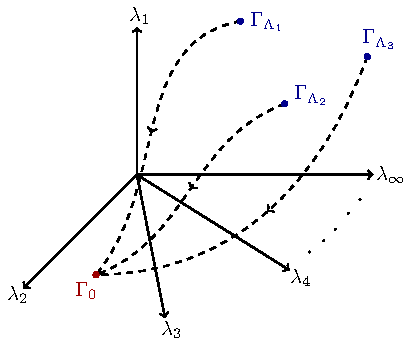
\includegraphics{figs/TikZ/regulator_dependence}
\caption[Flow of $\Gamma_k$ through infinite-dimensional theory space for different regulators.]{Flow of $\Gamma_k$ through infinite-dimensional theory space for different regulators, inspired by \cite{Gies2006}. Although the trajectories in theory space, governed by the flow equation (\ref{eqn:Wetterich}) may be different, they flow towards the same quantum effective action $\Gamma_{k\rightarrow 0} \equiv \Gamma$.}	
\label{fig:theory_space}
\hrulefill
\end{figure}
It is important to mention, that the Wetterich equation is an \textit{exact} equation, no approximations have been made. The only modification, the implementation of $\Delta S_k$ vanishes in the limit $k\rightarrow 0$. Solutions of the flow equation correspond to trajectories in \textit{theory space}, the space spanned by all (= infinitely many) dimensionless couplings $g_{\alpha}$. The choice of the regulator has direct impact on the exact form of the trajectory. This is often referred to as \textit{scheme dependence}. Nevertheless, for all regulators satisfying the properties (\ref{eqn:regulator_limits}) it is guaranteed, that the flow will lead to the same quantum effective action $\Gamma$. For a visualization of this idea, have a look at figure (\ref{fig:theory_space}).  In principle this means, that $\lim_{k\rightarrow 0}\Gamma_k\equiv\Gamma$, but in most practical cases it is unavoidable to employ truncation schemes to be able to solve the flow equation. A plethora of different truncation schemes has been developed recently, details concerning the most important schemes can be found e.\,g. in the reviews about the FRG we referred to at the beginning of this section. We want to conclude this chapter with a more formal discussion of the concept of theory space, before proceeding to an introduction of the basic concepts of (classical) gravity.
\section{Renormalization Group Flow and Theory Space}
We want to use this section to formalize the concept of theory space we introduced in the last section and to discuss important characteristics of the renormalization group flow such as the beta functions and their zeros, the fixed points of the flow. For this part, we mainly follow \cite{ReuterSaueressig2012}. \\
The theory space is defined as the space spanned by all dimensionless couplings of the theory. To be more precise, it consists of all (action) functionals $A:\Phi \mapsto A[\Phi]$, that are compatible with the imposed symmetries of the theory such as e.\,g. diffeomorphism invariance in the case of (quantum) gravity. \\
The flow equation (\ref{eqn:Wetterich}) defines a vector field $\vec{\beta}$ in theory space whose integral curves are the trajectories $\Gammak$ parametrized by the scale $k$. Assuming the existence of a complete set of basis functionals $\left\{P_{\alpha}[\ \cdot \ ]\right\}$, we can expand $\Gamma_k$ as follows:
\begin{equation}
	\Gamma_{k}[\Phi, \bar{\Phi}]=\sum_{\alpha=1}^{\infty} \bar{g}_{\alpha}(k) P_{\alpha}[\Phi, \bar{\Phi}].
\end{equation}
Here, the expansion coefficients $ \bar{g}_{\alpha}(k)$ are given by the generalized couplings. Inserting this ansatz into the flow equation (\ref{eqn:Wetterich}), yields a set of infinitely many coupled differential equations for the couplings:
\begin{equation}
	k \partial_{k} \bar{g}_{\alpha}(k)=\bar{\beta}_{\alpha}\left(\bar{g}_{1}, \bar{g}_{2}, \cdots ; k\right), \qquad \alpha=1,2, \cdots
\end{equation}
The \textit{beta functions} $\bar{\beta}_{\alpha}\left(\bar{g}_{1}, \bar{g}_{2}, \cdots ; k\right)$  are the components of the vector field $\vec{\beta}$ and arise from an expansion of the trace on the r.\,h.\,s. of the flow equation in terms of the functional basis\footnote{The expansion reads: $\frac{1}{2}\tr{\cdots} = \sum_{\alpha=1}^{\infty} \bar{\beta}_{\alpha}\left(\bar{g}_{1}, \bar{g}_{2}, \cdots ; k\right) P_{\alpha}[\Phi, \bar{\Phi}]$.}. Up to this point, we are still dealing with dimensionful couplings $\bar{g}$, but as mentioned earlier usually the flow equation is expressed in terms of \textit{dimensionless couplings}
\begin{equation}
	g_{\alpha} \equiv k^{-d_{\alpha}} \bar{g}_{\alpha},
\end{equation}
where $d_{\alpha}$ is the canonical mass dimension of the respective coupling. The \textit{essential} couplings\footnote{Essential in this sense means, that they can not be absorbed into the fields via a rescaling.} provide a set of coordinates for the theory space. This allows us to interpret the idea of renormalization theory in a new, geometrical way: We need to construct \enquote{infinitely long} trajectories $\Gammak$, that lie \textit{entirely} in theory space. In this case, the couplings are prevented from diverging and we are able to define a consistent quantum field theory. \newpage
A \textit{fixed point} $g^{*}$ of the flow is a zero point of the vector field $\vec{\beta}$, i.\,e.  $\beta_{\alpha}(g^{*})\equiv 0 \ \forall \alpha$. The existence of such fixed points is crucial for our discussion of Asymptotic Safety as an approach to quantum gravity, based on the concepts we introduced here. \\
\begin{figure}[t]
	\centering
	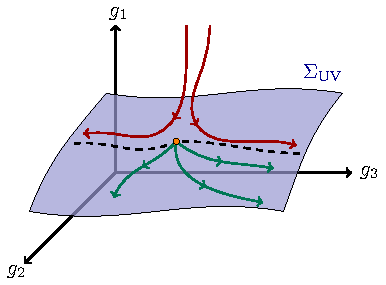
\includegraphics[width=0.5\textwidth]{figs/TikZ/hypersurface}
	\caption[Visualization of a fixed point with its corresponding UV hypersurface $\Sigma_{\mathrm{UV}}$ in theory space.]{Visualization of a fixed point $g^{*}$ (orange dot) with its corresponding UV hypersurface $\Sigma_{\mathrm{UV}}$ and trajectories starting at $g^{*}$ (green) in theory space. The flow points towards the IR. Trajectories starting off the surface (red) are pulled towards the FP along the irrelevant direction (here: $g_1$) until  the IR repulsive directions $g_2$ and $g_3$ dominate and drive the flow away from $g^{*}$. This figure is inspired by \cite{Eichhorn2018}.}\label{fig:hypersurface}
	\hrulefill
\end{figure}
In general, one distinguishes different classes of fixed points. The \textit{Gaussian} or \textit{non-inter-acting} fixed points  (GFP) are classified by $g^{*}_{\alpha}=0 \ \forall\alpha$. This class of fixed points is relevant for perturbation theory, where the limit $k\rightarrow\infty$ is taken at such a GFP\footnote{E.\,g. in Yang-Mills theory, the concept of \textit{Asymptotic freedom}, where the couplings tend to zero in the limit $k\rightarrow\infty$, is based on the existence of an UV attractive Gaussian fixed point, rendering the theory perturbatively renormalizable \cite{GrossWilczek1973}.}. If at least one of the couplings $g^{*}_{\alpha}\neq 0$, the fixed point is classified as \textit{Non-Gaussian} or \textit{interacting} (NGFP). The idea of Asymptotic Safety relies on the existence of such a NGFP, rendering the theory \enquote{safe} from divergences in the ultraviolet (UV) regime. An important characteristic of a fixed point is its stability or more precisely if it is \textit{attractive} or \textit{repulsive} for near RG trajectories. Additionally one distinguishes between infrared ($k\rightarrow0$) and ultraviolet ($k\rightarrow\infty$) attractive (repulsive) fixed points. To analyze this behavior, the flow near a fixed point is linearized, i.\,e.
\begin{equation}
	\partial_{t} g_{\alpha}(k)=\sum_{j=1}^{\infty} B_{\alpha j}\left(g_{j}-g_{j}^{*}\right),
	\label{eqn:linearized_flow}
\end{equation}
where we defined the \textit{stability matrix} \ $\mathbf{B} = B_{\alpha j} = \partial_j\beta_{\alpha}(g^{*}_{\alpha}) $. The solution of the differential equation (\ref{eqn:linearized_flow}) reads:
\begin{equation}
	g_{\alpha}(k)=g_{\alpha}^{*}+\sum_{j=1}^{\infty} C_{j} V_{\alpha}^{j}\left(\frac{k}{k_{0}}\right)^{\theta_{j}}.
\end{equation}
Here, the $V^{j}$ are the eigenvectors of the stability matrix with eigenvalues $\theta_j$ a.\,k.\,a. \textit{critical exponents}. In general, the $\theta_{j}$, are complex numbers. We use the real part of the critical exponents to classify the coupling as \textit{relevant} (= attractive) or \textit{irrelevant} (= repulsive):
\begin{align}
	g^{*}_{\alpha} \ \text{ is } \left\{\begin{array}{ll}{\text{relevant }} & {\text { for } \ \mathfrak{Re}\left(\theta_j\right) > 0} \\[10pt] {\text{irrelevant }} & {\text { for } \  \mathfrak{Re}\left(\theta_j\right) < 0} \\ \end{array}\right..
\end{align}
Fixed points with critical exponents $\theta_{j}=0$ are called \textit{marginal}. Based on this classification, it follows quite naturally to define an UV (or IR)  \textit{critical hypersurface} $\Sigma_{\mathrm{UV}}$ in theory space for a NGFP, consisting of all points that are pulled into the NGFP for increasing $k$. The dimension of $\Sigma_{\mathrm{UV}}$ is equal to the number of UV relevant couplings. This means, that trajectories lying on such a hypersurface tend to flow towards the fixed point in the UV limit. To visualize this idea, a schematic sketch of such a hypersurface in a $3$-dim. theory space is depicted in figure (\ref{fig:hypersurface}).
	\chapter{Curved Spacetimes and Gravity}\label{chap:GR}
Our current understanding of gravity is manifested in Einsteins theory of General Relativity. Different to the treatment of the other fundamental forces, all described by gauge theories and summarized in the Standard Model of Particle Physics, gravity is based on the concept of curved spacetime. This chapter summarizes some of the general concepts and notions of General Relativity, needed for a basic understanding of the subject. For most of the concepts we present here, we are following Sean Carrolls lecture notes \cite{CarrollGR}. At the end of this chapter, we show why gravity can not be quantized in a perturbative manner, opposite to the other three fundamental forces. For this part, we follow \cite{PawlowskiNPgaugeLecture}. 

\section{An Introduction to Spacetime Geometry}
 When talking about the concept of curved spacetimes, one first needs a mathematical framework to quantify curvature and to understand how mathematical concepts such as differentiation and integration are generalized to curved spaces. 
 The central objects in our discussion of curved spaces are \textit{differentiable manifolds}, i\,e. topological spaces, that are  locally diffeomorphic to $\mathbb{R}^n$. Locally in this sense means, that we can find coordinate maps $\phi_i: M \underset{\mathrm{open}}{\supset} U_i \rightarrow \mathbb{R}^n$, such that the image $\phi_i(U_i)$ is open in  $\mathbb{R}^n$, for every point on $M$, whereas globally the manifold may have a very complicated topology. A set of such coordinate maps $\{(U_{\alpha}, \phi_{\alpha})\}$ that covers the entire manifold and where the charts are smoothly sewed together is called an \textit{atlas}. For overlapping charts $U_{\alpha}\cap U_{\beta} \neq \emptyset$, the maps $(\phi_{\alpha} \circ \phi_{\beta}^{-1})$, a.\,k.\,a. coordinate transformations, must be smooth and differentiable. They are directly connected to the coordinates $x^{\mu}$ we'll work with later on. \\
Further, we need to introduce additional structures, such as vectors and tensors on manifolds, since they are the objects we are interested in when it comes to the discussion of physical models. To be able to talk about vectors, one needs to associate  a \textit{tangent space} $T_p$ to every point $p$ of the manifold. The tangent space is the set of all vectors at  $p$ and  has the structure of a vector space with the same dimension as $M$. The disjoint union of all tangent spaces on $M$ is called the \textit{tangent bundle}. To specify the concept of the tangent space we claim, that it can be identified with the space of directional derivative operators along curves $\gamma: \mathbb{R} \rightarrow M$  through $p$. In this case, we find a basis of $T_p$ as the set $\{\hat{\partial}_{\mu}\}$ of directional derivatives at $p$. It can be shown, that the directional derivatives can be decomposed into a sum of real numbers times partial derivatives, i.\,e. $\frac{d}{d \lambda} = \frac{d x^{\mu}}{d \lambda}\partial_{\mu}$, where $\lambda$ is the parameter of the curve $\gamma$. This allows us to represent a vector $V=V^{\mu}\partial_{\mu}$ independent of the chosen coordinates. The basis vectors in some different coordinate system $x^{\mu^{\prime}}$ are then simply related to the initial basis via $\partial_{\mu^{\prime}}=\frac{\partial x^{\mu}}{\partial x^{\mu^{\prime}}} \partial_{\mu}$ which yields the transformation law for vector components under general coordinate transformations,
\begin{align}
	V^{\mu^{\prime}}=\frac{\partial x^{\mu^{\prime}}}{\partial x^{\mu}} V^{\mu}. \label{eqn:contravariant_trafo}
\end{align}
Components obeying this transformation law are called \textit{contravariant}. At this point it follows quite naturally to define the \textit{cotangent space} $T_p^*$ as the set of linear maps $\omega: T_p \rightarrow \mathbb{R}$. Elements of the cotangent space are called one-forms or dual vectors and similarly to the discussion of the tangent space, we find a suitable basis for $T_p^*$ as the gradients $\{\dd\hat{x}^{\mu}\}$, allowing us to represent arbitrary one-forms as $\omega = \omega_{\mu} \dd x^{\mu}$. As before, we are interested in the transformation behavior of our basis one-forms, i.\,e. $\mathrm{d} x^{\mu^{\prime}}=\frac{\partial x^{\mu^{\prime}}}{\partial x^{\mu}} \mathrm{d} x^{\mu}$ and the dual vector components
\begin{align}
	\omega_{\mu^{\prime}}=\frac{\partial x_{\mu}}{\partial x^{\mu^{\prime}}} \omega_{\mu}.\label{eqn:covariant_trafo}
\end{align}
This transformation behavior differs from the one found for vectors. We call components transforming as in equation (\ref{eqn:covariant_trafo}) \textit{covariant}.
Now we are able to generalize these concepts by introducing tensors $T$ of type $(k,l)$ as
\begin{align}
T=T_{\phantom{\mu_{1} \cdots \mu_{k}}\nu_{1} \cdots \nu_{l}}^{\mu_{1} \cdots \mu_{k}} \ \partial_{\mu_{1}} \otimes \cdots \otimes \partial_{\mu_{k}} \otimes \mathrm{d} x^{\nu_{1}} \otimes \cdots \otimes \mathrm{d} x^{\nu_{l}}.
\end{align}
Here $\otimes$ denotes the usual tensor product.
The general transformation law for tensors follows naturally as expected from equations (\ref{eqn:contravariant_trafo}) and (\ref{eqn:covariant_trafo}),
\begin{align}
	T_{\phantom{\mu_{1}^{\prime} \cdots \mu_{k}^{\prime}}\nu_{1}^{\prime} \cdots \nu_{l}^{\prime}}^{\mu_{1}^{\prime} \cdots \mu_{k}^{\prime}}=\frac{\partial x^{\mu_{1}^{\prime}}}{\partial x^{\mu_{1}}} \cdots \frac{\partial x^{\mu_{k}^{\prime}}}{\partial x^{\mu_{k}}} \frac{\partial x^{\nu_{1}}}{\partial x^{\nu_{1}^{\prime}}} \cdots \frac{\partial x^{\nu_{l}}}{\partial x^{\nu_{l}^{\prime}}} T^{\mu_{1} \cdots \mu_{k}}_{\phantom{\mu_{1} \cdots \mu_{k}}\nu_{1} \cdots \nu_{l}}.
\end{align}
Having understood the basic structures and their respective behavior under coordinate transformations, we are now able to present some of the most important tensors in general relativity. \\
Maybe the most important object to quantify curved space is the \textit{metric tensor} $g_{\mu\nu}$\footnote{It is convenient to write the components $T_{\phantom{\mu_{1} \cdots \mu_{k}}\nu_{1} \cdots \nu_{l}}^{\mu_{1} \cdots \mu_{k}}$ when speaking about tensors $T$.} and its inverse  $g^{\mu\nu}$, related via $g^{\mu\nu}g_{\nu\sigma} = \delta^{\mu}_{\phantom{\mu}\sigma}$. The metric and its inverse can be used to raise and lower indices, e.\,g. $x^{\mu} = g^{\mu\nu}x_{\nu}$. Additionally we can compute path lengths and proper time via the definition of the line element 
\begin{align}
	d s^{2}=g_{\mu \nu} \mathrm{d} x^{\mu} \mathrm{d} x^{\nu}.
\end{align}
For arbitrary vector fields $V$ and $W$ the scalar product induced by the metric tensor reads
\begin{align}
	g(V,W) = g_{\mu\nu}V^{\mu}W^{\nu} = V^{\mu}W_{\mu}= g^{\mu\nu}V_{\mu}W_{\nu} = V_{\mu}W^{\mu}.
\end{align}
We will see, that the metric tensor already contains all the information on the geometrical structure of the respective manifold we need to quantify curvature. Nevertheless, we first have to think about differentiation of general tensors again. \\
In flat space, the partial derivative is a map from $(k, l)$ to $(k, l+1)$ tensor fields satisfying linearity and the Leibniz product rule. We want to generalize this concept to curved space by introducing the \textit{covariant derivative} $\nabla$\footnote{In the context of quantum field theory, the gauge covariant derivative is often written as $D$. Nevertheless, throughout this thesis we will use $\nabla$ to indicate any kind of covariant derivative.}. Different to the usual partial derivative, the covariant derivative is independent on the chosen set of coordinates. Consider for example the covariant derivative of a vector field $V$, which can be written as a partial derivative plus some correction term due to its property to obey the Leibniz rule:
\begin{align}
\nabla_{\mu} V^{\nu}=\partial_{\mu} V^{\nu}+\Gamma_{\phantom{\nu}\mu \lambda}^{\nu} V^{\lambda}.
\label{eqn:cov_deriv}
\end{align}
Here, the correction term is specified by the so-called \textit{Christoffel symbols} a.\,k.\,a. \textit{connection coefficients}. They are determined by derivatives of the metric tensor:  
\begin{align}
\Gamma_{\phantom{\alpha}\mu \nu}^{\alpha}=\frac{1}{2} g^{\mu \lambda}\left(\partial_{\mu} g_{\nu \lambda}+\partial_{\nu} g_{\mu \lambda}-\partial_{\lambda} g_{\mu \nu}\right)\footnotemark.	
\end{align}
\footnotetext{This holds only true, if the connection is \textit{torsion free} i.\,e. $
T_{\phantom{\lambda}\mu \nu}^{\lambda}=\Gamma_{\phantom{\lambda}\mu \nu}^{\lambda}-\Gamma_{\phantom{\lambda}\nu \mu}^{\lambda}=2 \Gamma_{\phantom{\lambda}[\mu \nu ]}^{\lambda} = 0$ and fullfils \textit{metric compatibility} i.\,e.$
\nabla_{\rho} g_{\mu \nu}=0$. For the most important connection in the context of General Relativity, the \textit{Levi-Civita connection}, these properties are fullfilled. The fundamental theorem of Riemannian geometry states, that for every Riemannian manifold there exists a unique Levi-Civita connection. It is determined by the Koszul formula.}
It can be shown, that the connection coefficients themselves do \textit{not} transform like tensor components, but are constructed in a way such that the combination (\ref{eqn:cov_deriv}) does. Note, that the covariant derivative reduces to the partial when applied to scalars. With this definition of the connection, we are now finally able to introduce the remaining tensor structures needed for the understanding of the calculations presented later on in this work. \\
The central object in our discussion of curvature is the \textit{Riemann tensor} $R_{\phantom{\alpha}\beta \gamma \delta}^{\alpha}$. It is a $(1, 3)$-tensor given by
\begin{align} 
	R_{\phantom{\alpha}\beta \gamma \delta}^{\alpha}=\partial_{\gamma} \Gamma_{\phantom{\alpha}\beta \delta}^{\alpha}-\partial_{\delta} \Gamma_{\phantom{\alpha}\beta \gamma}^{\alpha}+\Gamma_{\phantom{\alpha}\beta \delta}^{\epsilon} \Gamma_{\phantom{\alpha}\epsilon \gamma}^{\alpha}-\Gamma_{\phantom{\alpha}\beta \gamma}^{\epsilon} \Gamma_{\phantom{\alpha}\epsilon \delta}^{\alpha}.
\end{align}
It contains all the information about the curvature of the respective manifold. Another useful definition of the Riemann tensor is related to the commutator of two covariant derivatives, acting on a vector field:
\begin{align}
	\left[\nabla_{\mu}, \nabla_{\nu}\right] A^{\sigma}=R_{\phantom{\alpha}\rho \mu \nu}^{\sigma} A^{\rho}. \label{eqn:Riemann}
\end{align}
We are also interested in contractions of the Riemann tensor, especially the \textit{Ricci tensor} 
\begin{align}
	R_{\mu\nu} = R^{\alpha}_{\phantom{\alpha}\mu\alpha\nu} = g_{\alpha\beta} R^{\beta}_{\phantom{\alpha}\mu\alpha\nu}
\end{align}
and the \textit{Ricci scalar} 
\begin{align}
\mathcal{R} = g_{\mu\nu}R^{\mu\nu} = R^{\mu}_{\phantom{\mu}\mu}.
\end{align}
At this point, we also want to introduce the \textit{Einstein tensor}, defined as
\begin{align}
	 G_{\mu\nu} = R_{\mu\nu} - \frac{1}{2}g_{\mu\nu}\mathcal{R}.
\end{align}
Having introduced the setup for the calculations performed in this work, we are now ready to introduce the \textit{Einstein-Hilbert action}, providing the starting point for an investigation of quantum gravity within the Functional Renormalization Group approach. 
\section{From Geometry to Einsteins Equations}
The Einstein-Hilbert action, given by
\begin{align}
	\mathcal{S}_{\text{EH}} = \frac{1}{16\pi G} \int_x \sqrt{g} \ (\Ricci - 2\Lambda), 
\end{align}
where $G$ is Newtons coupling and $\Lambda$ is the cosmological constant, describes a minimally coupled theory of gravity, leading to a $\sfrac{1}{r}$ gravitational potential in the non-relativistic limit. Note, that compared to the usual spacetime measure a factor of $\sqrt{g} := \sqrt{-\operatorname{det}g_{\mu\nu}}$ is included to preserve diffeomorphism invariance.\footnote{Diffeomorphism invariance, i.\,e. the freedom of choosing an appropriate coordinate system, is the central symmetry in the context of General Relativity, based  on the assumption, that coordinates do not exist a priori in nature, but are rather a mathematical tool used to describe it, that should not change the fundamental laws of physics.\nopagebreak} \\ 
Varying the Einstein-Hilbert action w.\,r.\,t. the inverse metric $g^{\mu\nu}$ yields Einsteins equations in absence of matter:
\begin{align}
	G_{\mu\nu} + \Lambda g_{\mu\nu} = 0.
\end{align}
The non-vacuum Einstein equations are obtained the same way, after the inclusion of matter in this setting  by adding a matter part to the Einstein-Hilbert action:
\begin{equation}
	\mathcal{S} = \frac{1}{8\pi G}\mathcal{S}_{\mathrm{EH}} + \mathcal{S}_{\text{matter}}.
\end{equation}
With the definition of the Energy-Momentum tensor $T_{\mu\nu}$, given by
\begin{align}
	T_{\mu\nu} = \frac{-2}{\sqrt{g}} \frac{\delta\mathcal{S}_{\text{matter}}}{\delta g^{\mu\nu}},
\end{align}
we arrive at 
\begin{align}
\frac{1}{8\pi G}\left[G_{\mu\nu} + \Lambda g_{\mu\nu}\right] = T_{\mu\nu}.	
\end{align}
In this form, Einsteins equations perfectly embody the direct correlation between curvature (l.\,h.\,s.) and the dynamics of the matter content of the theory (r.\,h.\,s.). \\
At the end of this chapter we want to emphasize the problem of perturbative non-renormali- zability in the context of finding a quantum field theoretical description of gravity. 
\section{Perturbative Non-Renormalizability of Gravity}
Naively, one could try to quantize gravity via the path integral formalism with a generating functional, given by $\int_{g_{\mu\nu}} \operatorname{e}^{-\mathcal{S}_{\mathrm{EH}}}$, as usual. The main problem in this approach is the lack of positivity of $\mathcal{S}_{\mathrm{EH}}$ causing problems with unitarity of the theory. In quantum gravity one usually introduces a linear split of the \textit{full} metric $g_{\mu\nu}$, to perform expansions about a given background $\bar{g}_{\mu\nu}$, comparable to classical perturbation theory, which is based on coupling or amplitude expansions about the free Gaussian theory. The linear split reads
\begin{align}
	g_{\mu\nu} = \bar{g}_{\mu\nu} + \sqrt{G}h_{\mu\nu},
\end{align}
with the metric fluctuation $h_{\mu\nu}$ defined as $h_{\mu\nu}= 1/\sqrt{G}\left(g_{\mu\nu}-\bar{g}_{\mu\nu}\right)$. This allows us to write the path integral in terms of the fluctuation field as
\begin{equation}
Z\left[J^{\mu \nu} ; \overline{g}_{\mu \nu}\right] \propto \int_{h_{\mu \nu}} \operatorname{e}^{-S_{\mathrm{EH}}\left[\overline{g}_{\mu \nu}+\sqrt{G} h_{\mu \nu}\right]+\int_x \sqrt{\bar{g}} \  J^{\mu \nu} h_{\mu \nu}}.
\end{equation}
Note, that the source term depends on the determinant of the background metric, otherwise the usual $J^{\mu\nu}$ derivatives would not generate the $n$-point functions of the fluctuation field $h_{\mu\nu}$. We will come back to this problem, which is often referred to as \textit{background independence}, at the end of this thesis in chapter \ref{chap:BGindependence}. \\
After a suitable tensor decomposition of the fluctuation field and a gauge fixing procedure \`a la Faddeev-Popov\footnote{The functional quantization of gauge theories requires a gauge fixing procedure due to redundancies in the path integral measure. The idea of Faddeev and Popov is to represent the gauge fixing condition, which is implemented in the functional integral, as an additional functional integral over a set of Grassmann fields $c$ and $\bar{c}$, known as \textit{Faddeev-Popov ghosts}. Even though they are anticommuting Grassmann fields, they transform as scalars under Lorentz transformations. They also violate spin statistics. Nevertheless, they can be treated as additional particles in the computation of Feynman diagrams. For a detailed discussion, see e.\,g. ch. 16 in \cite{PeskinSchroeder1995} or  sec. 5.2 in \cite{PawlowskiNPgaugeLecture}.},  we are left with the gauge fixed Einstein-Hilbert action
\begin{align}
	\mathcal{S}_{\text{grav}}[\bar{g},\Phi] = \mathcal{S}_{\text{EH}}[g] + \mathcal{S}_{\text{gf}}[\bar{g}, h] + \mathcal{S}_{\text{gh}}[\bar{g},\Phi] .
\end{align}
 Here the pure gravity multi-field $\Phi=(h_{\mu\nu}, c_{\mu}, \bar{c}_{\mu})$ was introduced. All together, this yields the gauge-fixed path integral representation of quantum gravity:
 \begin{equation}
Z[J ; \bar{g}]=\int_{\Phi} \operatorname{e}^{-\mathcal{S}_{\text{grav}}\left[\bar{g}_{\mu\nu}, \Phi\right]+\int_x \sqrt{\bar{g}} \ J \cdot \Phi}.
\end{equation}
An analysis of the canonical momentum dimensions of the essential couplings of this theory, $G$ and $\Lambda$ results in:
\begin{equation}
\left[G\right] = \left[\dd^dx \sqrt{g}\ \mathcal{R}\right] = 2-d,  \qquad\qquad\qquad \left[\Lambda\right] = 2.
\end{equation}
This implies, that the Newton coupling has a negative mass dimension in $d=4$ spacetime dimensions. To investigate the consequences of this, one can consider the grade of divergence $\Lambda^{\delta(\gamma)}$ for a general graph $\gamma$ with $E$ external lines, $I$ internal propagators and $L$ loops. Here, $\Lambda$ is a UV cutoff for the momentum integrals and $\delta(\gamma)$ is the index of the graph,
\begin{equation}
	\delta(\gamma) = dL- 2\left(I-\sum_{n=3}^{\infty}\nu_n\right),
\end{equation}
where the $\nu_n$ represent $n$-graviton vertices. After expressing the number of loops in terms of the internal lines and the $n$-graviton vertices and restricting ourselves to graphs satisfying $E + 2I = \sum_{n=3}^{\infty}\nu_n$, we find
\begin{equation}
	\delta(\gamma)=d-\frac{d-2}{2} E+\sum\limits_{n=3}^{\infty} v_{n} \delta\left(v_{n}\right),
\end{equation}
where $\delta\left(v_{n}\right)=\frac{1}{2}(n-2)(d-2)$.
After fixing the number of external lines, e.\,g. to $E=2$, representing the case of vacuum polarizatio as depicted in figure (\ref{fig:vacuum_pol}), one is now able to investigate the grade of divergence for diagrams of different loop orders. t'Hooft and Veltman proved that the theory is renormalizable up to 1-loop order \cite{tHooftVeltmann1974}, but already at 2-loop order, Goroff and Sagnotti showed, that non-vanishing counterterms are generated \cite{GoroffSanotti1985}. In general, this is interpreted as the failure of perturbative quantization of gravity due to the negative mass dimension of the Newton coupling. This leads us to our discussion of Asymptotic Safety as a non-perturbative approach based on the functional renormalization group methods we presented in the last chapter.  

\begin{figure}[t]
\centering
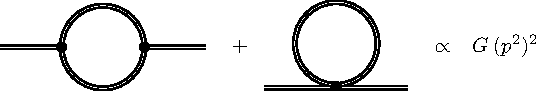
\includegraphics[width=0.8\textwidth]{figs/TikZ/vacuum_pol}
\caption[Vacuum polarization diagrams up to $1$-loop order.]{Vacuum polarization diagrams up to $1$-loop order. The double lines represent the graviton propagator.}	
\label{fig:vacuum_pol}
\hrulefill
\end{figure}
	\chapter{Functional Renormalization and Quantum Gravity}\label{chap:EHT}
In this chapter, we 
\section{Asymptotic Safety}
\begin{itemize}
	\item Taking the UV limit ..
\end{itemize}
\section{Einstein-Hilbert Truncation}

We want to solve the Flow equation ()%TODO: define QG flow equation to refero to
approximately. All terms that are invariant under the imposed symmetry, i.\,e. invariant under diffeomorphism transformations need to be taken into account. \\

Easiest truncation takes only the scalar curvature $\mathcal{R}$ and the cosmological constant $\Lambda$ into account (No higher order terms \dots) and was performed by Martin Reuter in 1993 \cite{ReuterSaueressig2002}. \\


This full truncation reads
\begin{align}
	\Gammak = 2\kappa^2Z_k \int_x \sqrt{g} \ [-\mathcal{R} + 2\Lambda_k] + \mathcal{S}_{\text{gf}} + \mathcal{S}_{\text{gh}}.
\label{eqn:QGflow}
\end{align}
with 
\begin{align}
	\kappa^2 = \frac{1}{32\pi G}, \qquad\qquad G_k = GZ^{-1}_k
\end{align}



anomalous dimension: 
\begin{align*}
	\eta_g = -\frac{\partial_t Z_k}{Z_k} = -\partial_t \ln Z_k
\end{align*}

dimensionless renormalized cosmological constant:
\begin{align*}
	\lambda_k = \Lambdak k^{-2}
\end{align*}

dimensionless renormalized cosmological constant:
\begin{align*}
	g_k = G_k k^{d-2} = \frac{Gk^{d-2}}{Z_k}
\end{align*}

corresponding beta function:
\begin{align}
	\beta_g = \partial_t g_k = \left(d-2 + \eta_g\right)g_k
\end{align}

maximally symmetric space:
\begin{align}
	\bar{\mathcal{R}}_{\mu\nu} = \frac{1}{d} \ \bar{g}_{\mu\nu} \bar{\mathcal{R}}
\end{align}
\begin{align}
	\bar{\mathcal{R}}_{\mu\nu\rho\sigma} = \frac{1}{d(d-1)} \ (\bar{g}_{\mu\rho}\bar{g}_{\nu\sigma} - \bar{g}_{\mu\sigma}\bar{g}_{\nu\rho}) \bar{\mathcal{R}}
\end{align}

suitable tensor basis:

%TODO: Adapt this to the definition given in the Appendix 
As a first approximation, we only take the contribution from the spin-two graviton mode $h_{\mu\nu}^{\text{TT}}$ into account. This is motivated by the fact, that this mode carries the the most degrees of freedom.\\ %TODO: Extend this explanation (exercise sheet...)
In this setting, we want to solve the Wetterich equation (\ref{eqn:Wetterich}) by computing the l.\,h.\,s. and the r.\,h.\,s. separately and extract the $\beta$-functions for the Newton coupling $g_k$ and the cosmological constant $\lambda_k$ by a comparison of all terms of order $\sim\sqrt{g}$ and $\sim \sqrt{g} \ \mathcal{R}$. \\
In our spin-two graviton mode approximation, we don't have to deal with the gauge-fixing and ghost parts ocuring in the effective action. The simplified version of equation (\ref{eqn:QGflow}) reads
\begin{align}
	\Gamma_{k, h^{\text{TT}}} = 2\kappa^2Z_k \int_x \sqrt{g} \ [-\mathcal{R} + 2\Lambda_k].
\end{align}
We start by computing the transverse-traceless graviton two-point function
\begin{align}
\Gamma_{h^{\text{TT}}h^{\text{TT}}}^{(2)} = \frac{Z_k}{32\pi}\left(\bar{\Delta} - 2\Lambda_k+\frac{2}{3}\bar{\mathcal{R}}\right).
\end{align}
Using a regulator of the form
\begin{align}
R_k  = \eval{\Gamma_{h^{\text{TT}}h^{\text{TT}}}^{(2)}}_{\Lambda_k=\bar{\mathcal{R}}=0} \cdot r_k\left(\frac{\bar{\Delta}}{k^2}\right) = \frac{Z_k}{32\pi}\bar{\Delta}\left(\frac{k^2}{\bar{\Delta}}-1\right)\theta\left(1-\frac{\bar{\Delta}}{k^2}\right), \nonumber
\end{align}
with a Litim-type cutoff
\begin{align}
r_k(y) = \left(\frac{1}{y}-1\right)\Theta(1-y), \label{eqn:Litim}
\end{align}
as discussed in chapter (\ref{chap:QFT}), we are directly able to compute the l.\,h.\,s. of the Wetterich equation, i.\,e. the scale derivative of the effective average action:
\begin{align}
	\partial_{t}\Gamma_{k,h^{\text{TT}}} = 2\kappa^2 Z_k\int_x \sqrt{g} \left\{\eta_g\mathcal{R}+2\left(k^2(\partial_t\lambda_k) + \Lambda_k(2 - \eta_g)\right)\right\}
\end{align}
One can extract the $\beta$-function for the Newton coupling without performing the analysis of the Wetterich equation, i.\,e. 
\begin{align}
\beta_g = \partial_t g_k = \partial_t\left(\frac{G\cdot k^2}{Z_k}\right) = g_k\left(2+\eta_g\right).
\end{align}

The computation of the r.\,h.\,s. of the flow equation is more complicated because it involves the computation of a trace of a function depending on the Laplacian on a curved background. We can use heat-kernel techniques to solve such equations. Heat-kernel computations are based on a curvature expansion in powers of the curvature scaler $\mathcal{R}$. For more details, have a look at the appendix (\ref{sec:heat-kernel}). As a first step, we simplify the trace expression as much as possible.

\begin{align}
\operatorname{Tr}\left[\frac{1}{\Gammak^{(2)} + R_k}\partial_t R_k\right] & = \operatorname{Tr}\left[\frac{\partial_t\left(\frac{Z_k}{32\pi}\bar{\Delta}\right)r_k}{\left(\frac{Z_k}{32\pi}\right)\left(\bar{\Delta} - 2\Lambda_k + \frac{2}{3}\bar{\mathcal{R}}\right) + \left(\frac{Z_k}{32\pi}\bar{\Delta}\right) r_k}\right]	\nonumber \\
\phantom{.} \\
&= \operatorname{Tr}\left[\frac{\bar{\Delta}\left(\partial_t r_k - \eta_g r_k\right)}{\bar{\Delta}(1+r_k)-2\Lambda_k+\frac{2}{3}\bar{\mathcal{R}}}\right] \nonumber
\end{align}

We expand this expression around vanishing curvature and get
\begin{align}
\resizebox{.9 \textwidth}{!}{$
\operatorname{Tr}\left[\frac{1}{\Gammak^{(2)} + R_k}\partial_t R_k\right] = \operatorname{Tr}\left[\frac{\bar{\Delta}\left(\partial_t r_k - \eta_g r_k\right)}{\bar{\Delta}(1+r_k)-2\Lambda_k}\right] - \frac{2}{3}\bar{\mathcal{R}}\operatorname{Tr}\left[\frac{\bar{\Delta}\left(\partial_t r_k - \eta_g r_k\right)}{\left(\bar{\Delta}(1+r_k)-2\Lambda_k\right)^2}\right] + \mathcal{O}(\mathcal{R}^2)$
}
\end{align}
Now we are able to evaluate these two terms separately using heat-kernel techniques. One finds for the first term
\begin{align}
\operatorname{Tr}\left[\frac{\bar{\Delta}\left(\partial_t r_k - \eta_g r_k\right)}{\bar{\Delta}(1+r_k)-2\Lambda_k}\right] = \frac{1}{(4\pi)^2}\int_x \sqrt{g} \left[5\Phi_2^1(-2\Lambda_k) - \frac{5}{6}\bar{\mathcal{R}}\Phi^1_1(-2\Lambda_k)\right],
\end{align}
with the threshold functions 
\begin{align}
	\Phi_n^p(\omega) = \frac{1}{\Gamma(n)}\int_0^{\infty}\dd z \ z^{n-1} \frac{z(-2zr_k(z)-\eta_gr_k(z))}{(z(1+r_k(z))+\omega)^p}.
\end{align}
Analogously, the second term in our expansion reads
\begin{align}
	-\frac{2}{3}\bar{\mathcal{R}}\operatorname{Tr}\left[\frac{\bar{\Delta}\left(\partial_t r_k - \eta_g r_k\right)}{\left(\bar{\Delta}(1+r_k)-2\Lambda_k\right)^2}\right] = -\frac{10}{3}\frac{\bar{\mathcal{R}}}{(4\pi)^2}\int_x  \sqrt{g} \frac{1-\frac{\eta_g}{6}}{(1-2\lambda_k)^2}.
\end{align}
For the cosmological constant, comparing the $\int\sqrt{g}$ terms yields
\begin{align}
	\beta_{\lambda} = \partial_t\lambda_k = -4\lambda_k + \frac{\lambda_k}{g_k} \partial_t g_k + \frac{5}{4\pi}g_k\frac{1-\frac{\eta_g}{6}}{1-2\lambda_k},
\end{align}
where the anomalous dimension $\eta_g$ is determined by comparing the $\int\sqrt{g}\mathcal{R}$ terms:
\begin{align}
\eta_g = -\frac{5}{3\pi} \left(\frac{1-\frac{\eta_g}{4}}{1-2\lambda_k} + 2\frac{1-\frac{\eta_g}{6}}{(1-2\lambda_k)^2}\right).	
\end{align}

The solution of this system of coupled differential equations is evaluated using \verb|Python3| and \verb|Wolfram Mathematica|. We arrive at the following fixed point values for the Newton coupling and the cosmological constant:
\begin{align}
	(g_k^*, \lambda_k^*) = (0.86, 0.18).
\end{align}
The corresponding critical exponents, i.\,e. minus the eigenvalues of the stability matrix evaluated at the fixed point, are given by the complex conjugated pair
\begin{align}
	\theta_{1,2} = 2.9 \pm 2.6i. 
\end{align}

\begin{figure}[t]
\centering
	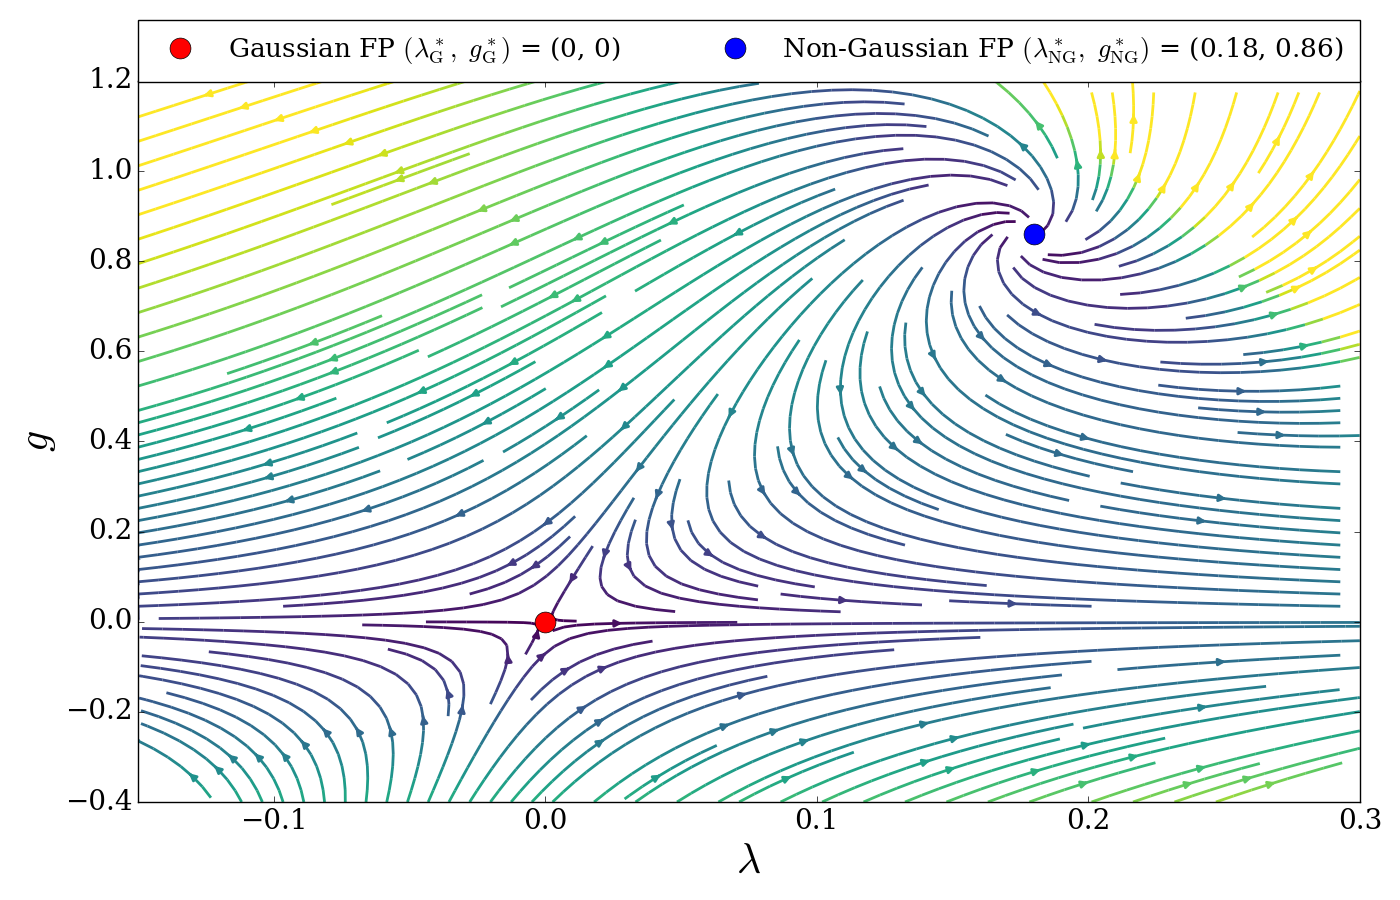
\includegraphics[width=\textwidth]{figs/Plots/EH_NoMatter}
	\caption[RG flow diagram for the Einstein-Hilbert truncation in TT approximation]{RG flow diagram  for the Einstein-Hilbert truncation in TT approximation as computed in this work. The flow points towards the infrared.}\end{figure}

%TODO: Interpretation and transition to next chapter (MATTER)
	\chapter{Asymptotic Safety of Gravity-Matter Systems}\label{chap:Matter}
For computing the contributions of the different matter fields on the running of the cosmological constant and the Newton coupling we follow \cite{DonaEichhornPercacci2013}. 


Some important formulas:
\begin{align}
	\eta_{\Psi} = -\partial_t \ln Z_{\Psi}
\end{align}

\begin{align}
	R_{k, \Psi}(z) = Z_{\Psi} \ \mathbbm{1} \ z \ r\left(\frac{z}{k^2}\right)
\end{align}
where $r$ is the same Litim-type shape function as defined in (\ref{eqn:Litim}).
\section{Matter Contributions from Background Field Computation}
\begin{align}
	\Gammak = \Gamma_{\text{EH}} + \mathcal{S}_{\text{gf}}+ \mathcal{S}_{\text{gh}}+ \Gamma_{\text{matter}}
\end{align}
where the different matter contributions come from
\begin{align}
	\Gamma_{\text{matter}} = \mathcal{S}_{\text{S}} + \mathcal{S}_{\text{D}} + \mathcal{S}_{\text{V}} 
\end{align}
with 
\begin{align}
	\mathcal{S}_{\text{S}} &= \frac{Z_{\text{S}}}{2}\int_x \sqrt{\operatorname{det}g} \ g^{\mu\nu} \ \sum\limits_{i=1}^{N_{\text{S}}} \partial_{\mu}\phi^{i}\partial_{\nu}\phi^{i} \\
	\phantom{.}\nonumber\\
	\mathcal{S}_{\text{D}} &= iZ_{\text{D}}\int_x \sqrt{\operatorname{det}g} \ \sum\limits_{i=1}^{N_{\text{D}}} \bar{\psi}^{i}\slashed{\nabla}\psi^{i}\\
	\phantom{.}\nonumber\\
		\mathcal{S}_{\text{V}} &= \frac{Z_{\text{V}}}{4}\int_x \sqrt{\operatorname{det}g} \ \sum\limits_{i=1}^{N_{\text{V}}} g^{\mu\nu}g^{\kappa\lambda}F^{i}_{\mu\kappa}F^{i}_{\nu\lambda} \nonumber \\
		&+ \frac{Z_{\text{V}}}{2\xi}\int_x \sqrt{\operatorname{det}\bar{g}} \ \sum\limits_{i=1}^{N_{\text{V}}} \left(\bar{g}^{\mu\nu}\bar{D}_{\mu}A_{\nu}^{i}\right)^2  \\
		&+ \frac{1}{2}\int_x \sqrt{\operatorname{det}\bar{g}} \ \sum\limits_{i=1}^{N_{\text{V}}} \bar{c}_i(-\bar{D}^2)c_i \nonumber
\end{align}
\begin{figure}[H]
	\centering
	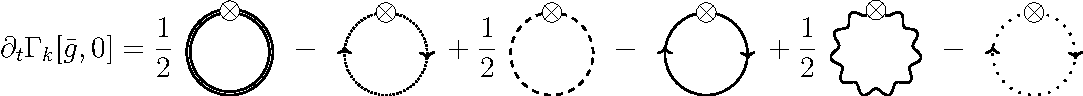
\includegraphics[width=0.95\textwidth]{figs/TikZ/matter_corrections}
	\caption[Flow equation for the average effective action $\Gamma_k$ including different matter contributions in diagrammatic representation.]{Flow equation for the average effective action $\Gamma_k$ including different matter contributions in diagrammatic representation. The double, dashed, solid and  wiggly lines correspond to the graviton, scalar, fermion and gauge field  propagators, respectively. The crossed circles denote the insertion of the respective regulator.}
\end{figure}

\begin{itemize}
	\item wo essential couplings, $G$ and $\Lambda$ and five inessential\footnote{Inessential in this sense means, that they can be eliminated by field rescalings.} wave function renormalizations $Z_{\Psi}$ with $\Psi = (h,c,S,D,V)$.
\end{itemize}
\subsection{Scalar fields}
\begin{align}
	\mathcal{S}_S &= \frac{Z_{S}}{2}\int_x \sqrt{\operatorname{det}g} \ g^{\mu\nu} \ \sum\limits_{i=1}^{N_{\text{S}}} \partial_{\mu}\phi^{i}\partial_{\nu}\phi^{i} \nonumber \\
&=  \frac{Z_{S}}{2}\int_x \sqrt{\operatorname{det}\bar{g}} \ \bar{g}^{\mu\nu} \ \sum\limits_{i=1}^{N_{\text{S}}} \partial_{\mu}\phi^{i}\partial_{\nu}\phi^{i} + \mathcal{O}(h) \\
&\overset{(\star)}{=} \frac{Z_{S}}{2}\int_x \sqrt{\operatorname{det}\bar{g}} \ \ \sum\limits_{i=1}^{N_{\text{S}}} \phi^{i}\left(-\bar{\nabla}^2\right)\phi^{i} + \mathcal{O}(h) \nonumber
\end{align}

Two-point function:
\begin{align}
	\Gamma^{(2)}_{\phi\phi} = \frac{\delta^2 \mathcal{S}_S}{\delta\phi^{i}\ \delta\phi^{j}} = Z_S \cdot\bar{\Delta}\cdot\mathbbm{1}_S + \mathcal{O}(h)  
\end{align}

Regularized Two-Point-Function:
\begin{align}
	\Gamma^{(2)}_{k, \phi\phi} = \left[\Gamma^{(2)}_{\phi\phi}+ R_{k, S}\right]  = Z_S \cdot\bar{\Delta}\cdot\mathbbm{1}_S\left(1 + r_k\left(\frac{\bar{\Delta}}{k^2}\right)\right) 
\end{align}



RHS of the flow equation:
\begin{align}
	\frac{1}{2}\tr{\left(\Gamma^{(2)}_{k, \phi\phi}\right)^{-1}\partial_t R_{k,S}} &= \frac{1}{2}\tr{\frac{Z_S\bar{\Delta}\left(\partial_t r_k - \eta_s r_k\right)}{Z_S \bar{\Delta}\left(1 + r_k\right)}\mathbbm{1}_S} \nonumber\\
	\phantom{.} \\
	&=   \frac{N_S}{2}\tr{\frac{\bar{\Delta}\left(\partial_t r_k - \eta_s r_k\right)}{\bar{\Delta}\left(1 + r_k\right)}} \nonumber
\end{align}

\subsection{Fermionic  fields}

\subsection{Gauge fields}
\begin{align}
	\mathcal{S}_{V, \mathrm{tot}} &= \frac{Z_{\text{V}}}{4}\int_x \sqrt{\operatorname{det}g} \ \sum\limits_{i=1}^{N_{\text{V}}} g^{\mu\nu}g^{\kappa\lambda}F^{i}_{\mu\kappa}F^{i}_{\nu\lambda}  
		+ \frac{Z_{\text{V}}}{2\xi}\int_x \sqrt{\operatorname{det}\bar{g}} \ \sum\limits_{i=1}^{N_{\text{V}}} \left(\bar{g}^{\mu\nu}\bar{D}_{\mu}A_{\nu}^{i}\right)^2  \nonumber\\
		&+ \frac{1}{2}\int_x \sqrt{\operatorname{det}\bar{g}} \ \sum\limits_{i=1}^{N_{\text{V}}} \bar{c}_i(-\bar{D}^2)c_i 
\end{align}



standard gauge field term:
\begin{align}
\mathcal{S}_{V} &=  \frac{Z_V}{4}\int_x \sqrt{\operatorname{det}g} \ \sum\limits_{i=1}^{N_{\text{V}}} g^{\mu\nu}g^{\kappa\lambda}F^{i}_{\mu\kappa}F^{i}_{\nu\lambda} \nonumber \\
&=  \frac{Z_{V}}{4}\int_x \sqrt{\operatorname{det}\bar{g}} \ \sum\limits_{i=1}^{N_{\text{V}}} \bar{g}^{\mu\nu}\bar{g}^{\kappa\lambda}\bar{F}^{i}_{\mu\kappa}\bar{F}^{i}_{\nu\lambda} + \mathcal{O}(h) \\
&\overset{(\ref{eqn:FF2})}{=} \frac{Z_{V}}{2}\int_x \sqrt{\operatorname{det}\bar{g}} \ \sum\limits_{i=1}^{N_{\text{V}}} A_{\lambda}^{i}\left[ \bar{\nabla}^{\mu}\bar{\nabla}^{\lambda} + \bar{g}^{\mu\lambda}\bar{\Delta}\right]A_{\mu}^{i} + \mathcal{O}(h) \nonumber
\end{align}
%TODO: Fix reference
gauge fixing term:
\begin{align}
	\mathcal{S}_{V, \mathrm{gf}} &= \frac{Z_{\text{V}}}{2\xi}\int_x \sqrt{\operatorname{det}\bar{g}} \ \sum\limits_{i=1}^{N_{\text{V}}} \left(\bar{g}^{\mu\nu}\bar{\nabla}_{\mu}A_{\nu}^{i}\right)^2  \nonumber\\
	&= \frac{Z_{\text{V}}}{2\xi}\int_x \sqrt{\operatorname{det}\bar{g}} \ \sum\limits_{i=1}^{N_{\text{V}}} \bar{g}^{\mu\nu}\bar{\nabla}_{\mu}A_{\nu}^{i}g^{\kappa\lambda}\bar{\nabla}_{\kappa}A_{\lambda}^{i} \\
	&\overset{(\star)}{=} \frac{Z_{\text{V}}}{2\xi}\int_x \sqrt{\operatorname{det}\bar{g}} \ \sum\limits_{i=1}^{N_{\text{V}}} A_{\lambda}^{i}\left[-\bar{\nabla}^{\lambda}\bar{\nabla}^{\mu}\right]A_{\mu}^{i} \nonumber
\end{align}
Both together 
Ghosts have to be considered separately \dots


\section{Perturbative Approximation}

\section{Some Words on Fermionic fields}
This section is mainly based on \cite{LippoldtPHD}  where the spin-base invariant formalism for treating fermions in curved spacetimes has been developed. The goal of this part of the thesis is to get a rough idea on how to perform calculations involving Dirac fermions, especially in the context of Asymptotic Safety of gravity-matter systems.  

Covariant derivative:
\begin{align}
	\nabla_{\mu} = \partial_{\mu} + \frac{1}{8}\left[\gamma^{a}, \gamma^{b}\right]\omega_{\mu}^{ab}
\end{align}


 \begin{figure}[t]
 \centering
 \hfill
 \begin{subfigure}{0.3\textwidth} 
	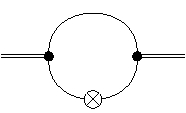
\includegraphics[width=\textwidth]{figs/TikZ/fermion_contribution}
 	\subcaption{Fermions.}
 \end{subfigure}
 \hfill
 \begin{subfigure}{0.3\textwidth} 
 	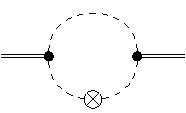
\includegraphics[width=\textwidth]{figs/TikZ/scalar_contribution}
 	\subcaption{Scalars.}
 \end{subfigure} 
 \hfill
 \begin{subfigure}{0.3\textwidth} 
 	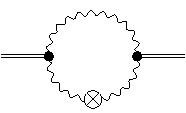
\includegraphics[width=\textwidth]{figs/TikZ/gauge_field_contribution}
 	\subcaption{Gauge Fields.}
 \end{subfigure} 
 \hfill
 \caption{Different matter contributions to the graviton anomalous dimension $\eta_h$.}	
 \end{figure}
 

 
  \begin{figure}[t]
 \centering
 \hfill
 \begin{subfigure}{0.3\textwidth} 
	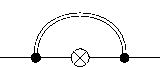
\includegraphics[width=\textwidth]{figs/TikZ/graviton_fluctuations1}
 \end{subfigure}
 \hfill
 \begin{subfigure}{0.3\textwidth}
 \vspace{-3.5pt}
 	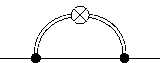
\includegraphics[width=\textwidth]{figs/TikZ/graviton_fluctuations2}
 \end{subfigure} 
 \hfill
 \begin{subfigure}{0.3\textwidth} 
 	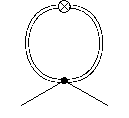
\includegraphics[scale = 1.5]{figs/TikZ/graviton_fluctuations3}
 \end{subfigure} 
 \hfill
 \caption[Contributing diagrams to the fermion anomalous dimension $\eta_D$.]{Contributing diagrams to the fermion anomalous dimension $\eta_D$. Analogous contributions arise for external scalars and gauge fields to $\eta_S$ and $\eta_V$.} 	
 \end{figure}
 
 \section{Background Field versus Fluctuation Field Calculation}

 
	\chapter{Conclusion}\label{chap:Conclusion}
In this thesis, we investigated the Asymptotic Safety scenario for quantum gravity and studied its phase diagram within the Einstein-Hilbert truncation in a background field approximation. We used non-perturbative Functional Renormalization Group techniques to compute the running of Newton's constant $g_k$ and of the cosmological constant $\lambda_k$.  \\

In chapters 1 to 3 we introduced the background knowledge, needed for a general understanding of the conducted calculations. After briefly discussing the general idea of the Asymptotic Safety conjecture, in chapter \ref{chap:EHT} we solved the flow equation for a pure-gravity system in a transverse-traceless spin-two graviton approximation to get a first insight into the underlying structures of the theory setting. The mathematical tools we used to solve the flow equation, such as the York decomposition of the fluctuation field and the heat-kernel techniques to compute the functional traces, were introduced very detailed. We computed the $\beta$-functions for $g_k$ and $\lambda_k$ and determined the fixed points of the flow. Besides the non-interacting Gaussian fixed point at $(g_k, \lambda_k)=(0, 0)$ we found an UV-attractive fixed point at $(g_k, \lambda_k)=(0.86, 0.18)$, providing further evidence for the Asymptotic Safety scenario as a promising candidate for a non-perturbative renormalizable quantum field theory of gravity. In chapter \ref{chap:Matter} we extended our truncation: First of all, the previously neglected trace mode and the Faddeev-Popov ghosts associated with the graviton sector were included to complete the calculation from chapter \ref{chap:EHT}. Then we investigated the impact of minimally coupled scalars, fermions and gauge fields on the Non-Gaussian fixed point. We explained in full detail how to solve the functional traces for all three matter types separately and presented the most important and insightful steps. After finishing the computation of all contributions, we were able to determine the $\beta$-functions for $g_k$ and $\lambda_k$ as a function of the number of matter fields. Neglecting all the contributions from the different anomalous dimensions and expanding the $\beta$-functions in some neighborhood of the Gaussian fixed point up to second order in the couplings, we qualitatively analyzed the behavior of the values for both couplings. We found out, that for an increasing amount of scalar fields, the values of the couplings tend to increase drastically. The fermionic fields and especially the gauge fields seem to have a stabilizing effect on the system. These results are almost in agreement with the results from earlier investigations, where similar conventions have been chosen, see e.\,g \cite{DonaEichhornPercacci2013}.
At the end, in chapter \ref{chap:BGindependence}, we highlighted some problems associated with the background field approximation, e.\,g. the loss of background independence as a consequence of violating the Nielsen identities. \\

This work may not provide fundamentally new results, but it still demonstrates some of the central concepts and calculations related to the subject. Due to the fact, that we worked in a rather simple truncation and chose a Litim-type cutoff, we we able to solve all the problems in this thesis analytically. Interesting modifications of our setup could include the employment of more sophisticated regulators or the inclusion of higher-order curvature terms. Compared to more recent results, the outcomes of our calculations should be treated with care. Nevertheless, this thesis provides a suitable framework for further investigations of asymptotically safe quantum gravity. Based on our discussion in chapter \ref{chap:BGindependence}, one may consider abandoning the background field approximation in future projects. 



%Appendices
\appendix{
	\chapter{Mathematical Background}\label{chap:AppA}
In this part of the appendix we want to discuss some of the mathematical tools we used during the calculations presented in the scope of this thesis in a more formal manner. 
The part on the York decomposition is mainly inspired by \cite{Percacci2017}, whereas the conventions for the heat-kernel computations are taken from \cite{PawlowskiNPgaugeLecture} and extended for the matter part, using the conventions from \cite{CodelloPercacciRahmede2008}.

\section{York Decomposition}
In the discussion of gauge theories, it is often very useful to decompose the gauge field $A_{\mu}$ into transversal and longitudinal parts:
\begin{align}
	A_{\mu} = A_{\mu}^{\mathrm{T}} + \nabla_{\mu}\phi.
\end{align}
The transversal part is characterized by the fact, that $\nabla^{\mu}A_{\mu}^{\mathrm{T}} = 0$. Using this decomposition, we are able to separate the pure gauge spin-$0$ degrees of freedom from the physical ones, contained in the spin-$1$ part $A_{\mu}^{\mathrm{T}}$.\\
Assuming vanishing boundary terms, integration by parts allows us to change the integration variables in the functional integral, i.\,e.
\begin{align}
	\int_x \sqrt{g} \ A_{\mu}A^{\mu} = \int_x \sqrt{g} \ A_{\mu}^{\mathrm{T}}A^{\mathrm{T}, \mu} + \int_x \sqrt{g} \ \phi\left(-\nabla^2\right)\phi.
\end{align}
Note, that we have to take care of the Jacobian $J$ of this variable transformation:
\begin{align}
	\left(\dd A_{\mu}\right) \longrightarrow J\left(\dd A_{\mu}^{\mathrm{T}}\right)\left(\dd\phi\right).
\end{align}
To be able to determine the Jacobian for our transformation, the integration measure needs to be normalized. A quite convenient choice is to evaluate the Gaussian integral over the different fields $\psi$ and set the result to one:
\begin{align}\label{eqn:york_measure}
	\int\left(\dd\psi\right) \exp\left\{-\int\dd x \ \sqrt{g} \ \psi^2 \right\} = 1,
\end{align} 
where we are assuming an Euclidean signature and a curved background metric. With this condition we find:
\begin{align}
	1&=J \int\left(\dd A_{\mu}^{\mathrm{T}}\right) \operatorname{e}^{-\int \dd x \sqrt{g} \ A_{\mu}^{\mathrm{T}} A^{\mathrm{T}, \mu}} 
	\int(\dd\phi) \operatorname{e}^{-\int \dd x \sqrt{g} \  \phi\left(-\nabla^{2}\right) \phi} = J\left(\operatorname{det}_{\phi}^{\prime}\left(-\nabla^{2}\right)\right)^{-1/2}.
\end{align}
This allows us to determine the Jacobian $J$ as follows:
\begin{align}
	J = \left(\operatorname{det}_{\phi}^{\prime}\left(-\nabla^{2}\right)\right)^{1/2}.
\end{align}
The prime denotes the fact, that the zero mode has to be removed, when computing the determinant to obtain a consistent result. Physically this is in accordance with the fact, that a constant $\phi$ does not contribute to $A_{\mu}$.\\
%TODO: Some words on non-local redefinitions
Four our computation in chapters \ref{chap:EHT} and \ref{chap:Matter}, we were using the background field method, where we assume a linear split of the \textit{full} metric $g_{\mu\nu}$ into a background metric $\bar{g}_{\mu\nu}$ and a fluctuation field $h_{\mu\nu}$. There is an analogous way of decomposing the fluctuation field in the background field formalism. First, we split $h_{\mu\nu}$ into
\begin{align}
	h_{\mu\nu} = h_{\mu\nu}^{\mathrm{T}} + \frac{1}{d}\ \bar{g}_{\mu\nu}h,
\end{align} 
where $h_{\mu\nu}^{\mathrm{T}}$ is traceless, i.\,e. $\bar{g}^{\mu\nu}h_{\mu\nu}^{\mathrm{T}}=0$ and $h=\bar{g}^{\mu\nu}h_{\mu\nu}$. The traceless part can be further decomposed in flat space using the irreducible representations of the Lorentz group with spins 0, 1 and 2 respectively, but in our case a more sophisticated approach, the so-called \textit{York decomposition} is chosen:
\begin{align}
	h_{\mu\nu} = h_{\mu\nu}^{\text{TT}} + \bar{\nabla}_{\mu}\xi_{\nu} + \bar{\nabla}_{\nu}\xi_{\mu} + \left(\bar{\nabla}_{\mu}\bar{\nabla}_{\nu} - \frac{1}{d} \ \bar{g}_{\mu\nu}\bar{\nabla}^2\right)\sigma + \frac{1}{d} \ \bar{g}_{\mu\nu}h.
\end{align}
Here, $ h_{\mu\nu}^{\text{TT}}$ is a transverse-traceless, spin-2 degree of freedom, $\xi_{\mu}$ is transverse and carries a spin-1 d.\,o.\,f. and $\sigma$ and $h$ have spin-0. As before, we want to find the Jacobian $J$ for this variable transformation:
\begin{align}
	\left(\dd h_{\mu\nu}\right) \longrightarrow J	\left(\dd h_{\mu\nu}^{\mathrm{TT}}\right) \left(\dd\xi_{\mu}\right)\left(\dd\sigma\right)\left(\dd h\right).
\end{align}
This is again possible after specifying a suitable normalization of the functional measure as
\begin{align}
	\int (\dd h_{\mu\nu}) \exp\left\{-\mathcal{G}(h, h)\right\} = 1,
\end{align}
where $\mathcal{G}$ is an inner product in the space of symmetric two-tensors, defined as
\begin{equation}
\begin{aligned} 
\mathcal{G}(h, h)&= \int_x \sqrt{\bar{g}} \ \left(h_{\mu \nu} h^{\mu \nu}+\frac{a}{2} h^{2}\right) \\[10pt]
&= \int_x \sqrt{\bar{g}} \ \left[h^{\mathrm{TT}}_{\mu \nu} h^{\mathrm{TT}, \mu \nu}+2 \xi_{\mu}\left(-\bar{\nabla}^{2}-\frac{\bar{R}}{d}\right) \xi^{\mu}\right. \\
&+\left.\frac{d-1}{d} \sigma\left(-\bar{\nabla}^{2}\right)\left(-\bar{\nabla}^{2}-\frac{\bar{R}}{d-1}\right) \sigma+\left(\frac{1}{d}+\frac{a}{2}\right) h^{2} \right] 
\end{aligned}
\end{equation}
in the case of an Einstein type background metric\footnote{A metric is of Einstein type, if $R_{\mu\nu}$ is a constant multiple of $g_{\mu\nu}$, i.\,e. $R_{\mu\nu} = \frac{1}{d} \mathcal{R} g_{\mu\nu}$.}. This yields
\begin{align}
	J=\left(\operatorname{det}_{\xi}\left(-\bar{\nabla}^{2}-\frac{R}{d}\right)\right)^{1 / 2}\left(\operatorname{det}_{\sigma}^{\prime}\left(-\bar{\nabla}^{2}\right)\right)^{1 / 2}\left(\operatorname{det}_{\sigma}\left(-\bar{\nabla}^{2}-\frac{R}{d-1}\right)\right)^{1 / 2}.
\end{align}
Note, that the prime has the same meaning and physical interpretation as in the previous case: If $\sigma$ is constant, it does not contribute to $h_{\mu\nu}$. \\
 For both cases, the decomposition of the general gauge field and the York decomposition of the fluctuation field, appropriate rescalings of the fields $\phi$, $\xi_{\mu}$ and $\sigma$ respectively, help us to cancel the non-trivial Jacobians and to achieve, that all modes have the same mass dimension. For the sake of completeness, we present the rescaled versions of the fields:
 \begin{align}
\hat{\phi} &= \sqrt{-\nabla^2}\ \phi \\[10pt]
 \hat{\xi}_{\mu} &= \sqrt{-\bar{\nabla}^{2}-\frac{\bar{R}}{d}}\  \xi_{\mu} \\[10pt]
  \hat{\sigma} &= \sqrt{-\bar{\nabla}^{2}} \sqrt{-\bar{\nabla}^{2}-\frac{\bar{R}}{d-1}}\ \sigma. 
 \end{align}
 The resulting graviton two-point function, after decomposition of the fluctuation field has the following structure:
\begin{equation} \Gamma^{(2)}_{hh} = 
\begin{pmatrix}
\Gamma^{(2)}_{h^{\mathrm{TT}}h^{\mathrm{TT}}} & 0 & 0 & 0 \\[10pt]
0 & \Gamma^{(2)}_{\xi\xi}  & 0 & 0 \\[10pt]
0 & 0 & \Gamma^{(2)}_{h^{\mathrm{Tr}}h^{\mathrm{Tr}}}  & \Gamma^{(2)}_{h^{\mathrm{Tr}}\sigma} \\[10pt]
0 & 0 & \Gamma^{(2)}_{\sigma h^{\mathrm{Tr}}} & \Gamma^{(2)}_{\sigma\sigma} \\

\end{pmatrix}
\end{equation}
 This concludes our discussion of the York decomposition, as a useful tool to simplify calculations in the background field method.
 \newpage
 \section{Heat-Kernel Techniques}\label{sec:heat-kernel}
We use heat-kernel techniques to evaluate the r.\,h.\,s. of the flow equation (\ref{eqn:Wetterich}), where we need to compute the functional trace over functions depending on the Laplacian on a curved background. In general, the method can be understood as a curvature expansion about a flat background. \\
The general formula to compute such traces is given by
\begin{align}
	\operatorname{Tr} f(\Delta)= N \  \int\kern-1.3em\sum_{\ell} \rho(\ell) f(\lambda(\ell)),
	\label{eqn:heat-kernel}
\end{align}
with some normalization $N$, the spectral values $\lambda(\ell)$ and their corresponding multiplicities $\rho(\ell)$. \\
On flat backgrounds, the computation of (\ref{eqn:heat-kernel}) is simply a standard momentum integral, whereas on curved backgrounds, consider for example a four-sphere $\mathbb{S}^4$ with constant background curvature $r = \frac{\bar{\mathcal{R}}}{k^2} > 0$, the spectrum of the Laplacian is discrete and we need to sum over all spectral values. \\
For our example of $\mathbb{S}^4$, we have
\begin{align}
	\lambda(\ell) = \frac{\ell(3+\ell)}{12}r \qquad \text{and} \qquad \rho(\ell) = \frac{(2\ell + 3)(l+2)!}{6\ell!}.
\end{align}
The normalization is then given by the inverse of the four-sphere-volume $ \left(V_{\mathbb{S}^4}\right)^{-1} = \frac{k^4r^2}{384\pi^2}$. This leads us to the formula for our computation of the r.h.s. of the flow equation on a background with constant positive curvature:
\begin{align}
\operatorname{Tr} f(\Delta)=\frac{k^{4} r^{2}}{384 \pi^{2}} \sum_{\ell=0}^{\infty} \frac{(2 \ell+3)(\ell+2) !}{6 \ell !} f\left(\frac{\ell(3+\ell)}{12} r\right).
\end{align}
This is called spectral sum. For large curvatures $r$ the convergence of the series is rather fast, whereas in the limit $r\rightarrow 0$ one finds exponentially slow convergence.\\
The master equation for heat kernel computations reads
\begin{align}
	\operatorname{Tr} f(\Delta)=\frac{1}{(4 \pi)^{\frac{d}{2}}}\left[\mathbf{B}_{0}(\Delta) Q_{2}[f(\Delta)]+\mathbf{B}_{2}(\Delta) Q_{1}[f(\Delta)]\right]+\mathcal{O}\left(\mathcal{R}^{2}\right),
\label{eqn:master-eqn}
\end{align}
with the heat-kernel coefficients 
\begin{align}
	\mathbf{B}_{n}(\bar{\Delta})=\int_x  \sqrt{g} \  \operatorname{Tr} \mathbf{b}_{n}(\bar{\Delta})
\end{align}
and 
\begin{align}
	Q_{n}[f(x)]=\frac{1}{\Gamma(n)} \int \dd x \ x^{n-1} f(x).\label{eqn:Qfunc}
\end{align}
For computations on $\mathbb{S}^4$, the values for the heat kernel coefficients $\mathbf{B}_n(\bar{\Delta})$ are presented in the following.
\begin{table}[H]
	\centering
	\setlength{\tabcolsep}{5mm}
	\setlength\extrarowheight{2mm}
	\begin{tabular}{c | c c c}
	   & TT & TV & S\\ \hline
	   $\operatorname{Tr} \mathbf{b}_{0}$ & 5 &  3 & 1\\
	  $\operatorname{Tr} \mathbf{b}_{2}$ & $-\frac{5}{6}\mathcal{R}$ & $\frac{1}{4}\mathcal{R}$& $\frac{1}{6}\mathcal{R}$\\
	\end{tabular}
	\caption{Heat-kernel coefficients for transverse-traceless tensors (TT), transverse vectors (TV) and scalars (S) for computations on $\mathbb{S}^4$.}
\end{table}

The basic idea of the proof of equation (\ref{eqn:heat-kernel}) is based on the Laplace transform
\begin{align}
	f(\Delta) = \int_0^{\infty} \dd s \ \operatorname{e}^{-s\Delta}\tilde{f}(s).
\end{align}
We insert this definition of the Laplace transform into equation (\ref{eqn:heat-kernel}) and find
\begin{align}
	\operatorname{Tr} f(\Delta)=\int_{0}^{\infty} \dd s \ \tilde{f}(s) \operatorname{Tr} \operatorname{e}^{-s \Delta}.
\label{eqn:hk2}
\end{align}
The trace on the r.\,h.\,s. is explicitly the trace of the heat kernel. We expand this term as follows:
\begin{align}
	\operatorname{Tr} \operatorname{e}^{-s \Delta}=\frac{1}{(4 \pi)^{\frac{d}{2}}} \sum_{n=0}^{\infty} s^{\frac{n-d}{2}} \mathbf{B}_{n}(\Delta).
\end{align}
This is where the heat-kernel coefficients $\mathbf{B}_n$ become important. We proceed by inserting this expanded version of the heat-kernel trace into equation (\ref{eqn:hk2}) and find:
\begin{equation}
\begin{aligned} 
\operatorname{Tr} f(\Delta) &=\frac{1}{(4 \pi)^{\frac{d}{2}}} \sum_{n=0}^{\infty} \mathbf{B}_{n}(\Delta) \int_{0}^{\infty} \dd s \ s^{\frac{n-d}{2}} \tilde{f}(s) \\[10pt] 
&=\frac{1}{(4 \pi)^{\frac{d}{2}}} \sum_{n=0}^{\infty} \frac{1}{\Gamma\left(\frac{d-k}{2}\right)} \mathbf{B}_{n}(\Delta) \int_{0}^{\infty} \dd t \ t^{\frac{d-n}{2}-1} f(t) \\[10pt]
 &=\frac{1}{(4 \pi)^{\frac{d}{2}}} \sum_{n=0}^{\infty} \mathbf{B}_{n}(\Delta) Q_{\frac{d-n}{2}}[f(t)].
\end{aligned}
\end{equation}
This completes the derivation of the master equation (\ref{eqn:master-eqn}) for heat-kernel computations. Note, that we used the definition of the $Q$-functionals, given in equation (\ref{eqn:Qfunc}) and the relation $\int_{s} s^{-x} \tilde{f}(x)=\frac{1}{\Gamma(x)} \int_{z} z^{x-1} f(z)$.


When investigating matter fields, such as in chapter \ref{chap:Matter}, we often encounter kinetic operators of the form $\tilde{\Delta} = -\nabla^2\cdot\mathbbm{1} +  \mathbf{E}$, where $\mathbf{E}$ is a linear map acting on the spacetime and the internal indices of the fields. In this notation, $\mathbbm{1}$ has to be understood as the identity in the respective field space. \\
If $\left[\Delta, \mathbf{E}\right] = 0$\footnote{In the case of $\left[\Delta, \mathbf{E}\right] \neq 0$, there would be additional terms including (higher order) commutators of $\Delta$ and $\mathbf{E}$ due to the Baker-Campbell-Hausdorff formula.}, we can relate the coefficients of the modified Laplacian $\tilde{\Delta}$ and those of the initially considered operator $-\nabla^2$ via
\begin{align}
	\operatorname{Tr} \operatorname{e}^{-s\left(-\nabla^{2}+\mathbf{E}\right)}=\frac{1}{(4 \pi)^{\frac{d}{2}}} \sum_{k, l=0}^{\infty} \frac{(-1)^{\ell}}{\ell !} \int_x \sqrt{g} \ \operatorname{Tr} \mathbf{b}_{k}(\Delta) \mathbf{E}^{\ell} s^{k+\ell-2}.
\end{align}
This results in the following, modified values for the coefficients we are interested in:
\begin{equation}
\begin{aligned}
	\mathbf{b}_0 &= \mathbbm{1} \\[10pt]
	\mathbf{b}_2 &= \frac{\mathcal{R}}{6}\cdot\mathbbm{1} - \mathbf{E}.
	\label{eqn:coefficients}
\end{aligned}	
\end{equation}
For further study and a more general treatment of the modified Laplacians, including higher order coefficients,\ \cite{CodelloPercacciRahmede2008, Percacci2017} are recommended.
	\chapter{Additional calculations}\label{chap:AppB}
For the sake of completeness, we present some auxiliary calculations and important steps, that were used to obtain the results presented in scope of this work, but were in general too long or unsuitable to be included in the main part.
\section{Matter contributions}
During the computation of the gauge field contribution to the running of $G$ and $\Lambda$, we encounter the following term, which can be simplified a lot after a few manipulations:
\begin{align}\label{eqn:FF2} 
\int g^{\mu\nu}g^{\kappa\lambda} F_{\mu\kappa}F_{\nu\lambda} = \int F_{\mu}^{\phantom{\mu}\lambda}F_{\phantom{\mu}\lambda}^{\mu}	&= \int  F_{\mu\lambda}F^{\mu\lambda} \nonumber	\\
&= \int \left(\partial_{\mu}A_{\lambda} - \partial_{\lambda}A_{\mu}\right)F^{\mu\lambda} + \mathcal{O}\left(A^3\right)\nonumber \\
&\overset{(\star)}{=} \int 2\partial_{\mu}A_{\lambda} F^{\mu\lambda}\nonumber  \\
&=  \int 2\partial_{\mu}A_{\lambda}\left(\partial^{\mu}A^{\lambda} - \partial^{\lambda}A^{\mu}\right) \\
&= \int 2\left(\partial_{\mu}A_{\lambda}\partial^{\mu}A^{\lambda} - \partial_{\mu}A_{\lambda}\partial^{\lambda}A^{\mu}\right) \nonumber\\
&\overset{(\dagger)}{=} -\int 2\left( A_{\lambda}\partial^2A^{\lambda} - A_{\lambda}\partial_{\mu}\partial^{\lambda}A^{\mu}\right) \nonumber\\
&= \int 2A_{\lambda}\left[\partial^{\mu}\partial^{\lambda} - g^{\mu\lambda}\partial^2\right]A_{\mu}\nonumber 
\end{align}

For the first non-trivial step ($\star$) we use that $2\partial_{\mu}A_{\lambda} = \partial_{(\mu}A_{\lambda)} + \partial_{[\mu}A_{\lambda]}$, where $(\cdots)$ and $[\cdots]$ denote symmetrization and antisymmetrization w.\,r.\,t. the indices, respectively. The symmetric part vanishes due to the fact, that $F^{\mu\lambda}$ is antisymmetric under $\mu \rightleftharpoons \lambda$. This allows us to write $2\partial_{\mu}A_{\lambda}F^{\mu\lambda} = \partial_{[\mu}A_{\lambda]}F^{\mu\lambda} = \left(\partial_{\mu}A_{\lambda} - \partial_{\lambda}A_{\mu}\right)F^{\mu\lambda}$. The  second non-trivial step ($\dagger$) results from integrating by parts and assuming vanishing boundary terms. \\
Later on in the gauge field calculation, after specifying the gauge parameter $\xi=1$, we encounter a commutator of covariant derivatives acting on $A_{\mu}$. With the definition of the curvature tensor, given in equation (\ref{eqn:Riemann}), we find
\begin{equation}
\begin{aligned}
\left[\nabla^{\mu}, \nabla^{\lambda}\right]A_{\mu} &= R_{\mu}^{\phantom{\mu}\rho\mu\lambda}A_{\rho} \\
&= R^{\rho\lambda}A_{\rho} \label{eqn:RiemannB}
\end{aligned}	
\end{equation}
Now, one simply has to rename the dummy indices $\rho \rightleftharpoons \mu$ to find the wanted expression. 	
}


\cleardoublepage
\pagenumbering{Roman}
%References, Figures etc.
\thispagestyle{plain}
\addcontentsline{toc}{chapter}{References}
\nocite{*}
\printbibliography[title=References]
\cleardoublepage

{\hypersetup{linkcolor=black}
\listoffigures
\addcontentsline{toc}{chapter}{List of Figures}
}	
\cleardoublepage
\thispagestyle{plain}
\section*{Acknowledgements}
First and foremost i would like to thank my supervisor Prof. Jan M. Pawlowski for giving me the opportunity to work on my desired topic and for always finding the time to discuss about open questions and the physical concepts this work is based on. I learned a lot about theoretical physics and had the chance to get in contact with a very interesting, modern research topic. \\

I want to thank Prof. J\"org J\"ackel for his interest in this project and for agreeing to become the second referee for this thesis.


Maybe the most important new experience for me was to be part of a research group and i have to say that i had a really great time at Philosophenweg 12! I have to thank the whole Quantum Gravity group for the nice atmosphere and many interesting and helpful discussions. It is great to know, that everybody in the groups takes the time to answer your questions and is willing to help you!  

  Especially i would like to thank Gustavo Brito for all the interesting blackboard sessions, which improved  my understanding of the subject a lot. \dots 

%For careful proofreading and many ideas on how to improve this work i have to thank \{ INSERT NAMES \}. I would particularly like to  thank my friends Marie Wintergerst and Mercal Abdin for their interest and for many advices, that helped me to improve this thesis.

Not to forget, i have to thank all my friends for the amazing time we spent together during the last years.

Lastly, i thank my parents Marie-Paule and Bernd Kaltschmidt and my sister C\'{e}line for their constant support and for always helping me to pursue my dreams.  
 

\section*{Declaration of Authorship}
I hereby certify that this thesis has been composed by me and is based on my own work, unless stated otherwise.\\

Heidelberg, 8$^{\mathrm{th}}$ of July 2019 \hfill \rule{60mm}{.15mm} \par \vspace{-0.4cm}
\hfill Mathieu Kaltschmidt
%TODO: Insert correct date


\end{document} 